\documentclass[compress]{beamer}
\usepackage[brazil]{babel}
\usepackage[latin1]{inputenc}
\usepackage{amsmath}
\usepackage{graphicx}
\usepackage{listings}

%%%%%%%%%%%%%%%%%%%%%%%%%%%%%
% C O N F I G U R A � � E S %
%%%%%%%%%%%%%%%%%%%%%%%%%%%%%
\definecolor{listinggray}{gray}{0.9}
\definecolor{lbcolor}{rgb}{1,1,1}

\lstset{
	backgroundcolor=\color{lbcolor},
	tabsize=4,
	rulecolor=,
	language=matlab,
    basicstyle=\scriptsize,
    upquote=true,
    aboveskip={1.5\baselineskip},
    columns=fixed,
    showstringspaces=false,
    extendedchars=true,
    breaklines=true,
    prebreak = \raisebox{0ex}[0ex][0ex]{\ensuremath{\hookleftarrow}},
    frame=single,
    showtabs=false,
    showspaces=false,
    showstringspaces=false,
    identifierstyle=\ttfamily,
}

\renewcommand{\lstlistingname}{C�digo}
\renewcommand{\lstlistlistingname}{Lista de C�digos}

\usetheme{Ilmenau}
%vinho
%\usecolortheme[RGB={75,11,31}]{structure}
%verde
%\usecolortheme[RGB={35,75,11}]{structure}
%azul
\usecolortheme[RGB={12,67,102}]{structure}
\setbeamercovered{transparent}
\setbeamertemplate{blocks}[rounded][shadow=true]
\setlength{\tabcolsep}{1mm}
%\setbeamertemplate{footline}[frame number]
\setbeamertemplate{navigation symbols}{}
\setbeamertemplate{headline}[default]
\setbeamertemplate{footline}[default]
\setbeamertemplate{footline}{\hspace*{.5cm}\scriptsize{\hfill\vspace*{0.3cm}\insertframenumber\hspace*{.5cm}}}

\newenvironment{changemargin}[2]{%
  \begin{list}{}{%
    \setlength{\topsep}{0pt}%
    \setlength{\leftmargin}{#1}%
    \setlength{\rightmargin}{#2}%
    \setlength{\listparindent}{\parindent}%
    \setlength{\itemindent}{\parindent}%
    \setlength{\parsep}{\parskip}%
  }%
  \item[]}{\end{list}}

%%%%%%%%%%%
% C A P A %
%%%%%%%%%%%

%\title{T�cnicas de Planejamento para Gera��o de Planos de Execu��o em um Sistema Gerenciador de Fluxos de Trabalho Cient�fico}

\title{Um Modelo de Execu��o de Fluxos de Trabalho Cient�fico Utilizando T�cnicas de Planejamento Autom�tico}

\author{Diogo Cezar Teixeira Batista \\
       {\footnotesize\ttfamily diogoc@inf.ufpr.br} \\
       Orientador: Fabiano Silva \\
       {\footnotesize\ttfamily fabiano@inf.ufpr.br}
}

\institute{\large Universidade Federal do Paran� - UFPR}

\date{Curitiba - 2012}

\begin{document}

%%%%%%%%%%%%%%%%%%%%%%%%%%%%%%%%
% S L I D E S  I N I C I A I S %
%%%%%%%%%%%%%%%%%%%%%%%%%%%%%%%%

\begin{frame}
    \titlepage
\end{frame}

\begin{frame}[t,allowframebreaks]
    \frametitle{Agenda}
    \tableofcontents
\end{frame}


%%%%%%%%%%%%%%%%%%%%%
% C A P � T U L O S %
%%%%%%%%%%%%%%%%%%%%%

\section[Introdu��o]{Introdu��o}
\begin{frame}
    \frametitle{Introdu��o}
    \begin{itemize}

        \item <1-> Onde est� a p�gina que procuro em um site?

%        \item <1-> Grande n�mero de sistemas hiperm�dia;
%
%        \item <2-> Informa��es distribu�das desorganizadamente na Internet;
%
%        \item <3-> Sistemas de busca;
%
%            \begin{itemize}
%                \item <4-> Trazem conte�do n�o relacionado, ou
%                irrelevante (sem�ntica);
%                \item <5-> N�o oferecem assist�ncia navegacional;
%            \end{itemize}

        \item <2-> \emph{Hiperm�dia Adaptativa}: modifica��o do conte�do
        \emph{web}.

        \item <3-> Proposta: navega��o colaborativa;

            \begin{itemize}
                \item <4-> Ajuda m�tua entre os usu�rios que
                estiverem navegando pelas mesmas p�ginas;

                \item <5-> Solu��o baseada na teoria do comportamento das
                formigas;
            \end{itemize}

    \end{itemize}
\end{frame}

\section[Trabalhos Relacionados]{Trabalhos Relacionados}

\begin{frame}
    \frametitle{Trabalhos Relacionados}
    \begin{itemize}
		\item Ptolemy, 2003 e Kepler, 2004:
		\item Pegasus, 2004;
		\item SciCumulus, 2010;
		\item Dornemann, Juhnke, Noll, Seiler e Freisleben, 2010;
		\item Gil, Deelman, Blythe, Kesselman e Tangmunarunkit, 2004;
		\item Compara��es;
	\end{itemize}
\end{frame}

\begin{frame}
    \frametitle{Trabalhos Relacionados}
	\begin{itemize}
		\item Ptolemy/Kepler:
		\begin{itemize}
			\item implementa��o da mesma opera��o sobre dados de diferentes formas (atores);
			\item modelo � capaz de selecionar qual a melhor implementa��o do operador para a execu��o em quest�o;
		\end{itemize}
		\item Pegasus:
		\begin{itemize}
			\item sistema � realimentado com metadados coletados em suas execu��es;
		\end{itemize}
		\item SciCumulus:	
		\begin{itemize}
			\item inspirou a utiliza��o de paralelismo: sobre dados e sobre execu��o;
		\end{itemize}
	\end{itemize}
\end{frame}

\begin{frame}
    \frametitle{Trabalhos Relacionados e Compara��es}

	\begin{itemize}
		
		\item Dornemann at al, 2010:
		\begin{itemize}
			\item coletor de informa��es;
		\end{itemize}
		\item Gil at al, 2004:
		\begin{itemize}
			\item aprimora o escalonamento utilizando t�cnicas de planejamento;
		\end{itemize}
	\end{itemize}

	\scriptsize
	\begin{table}[!htb]
		\begin{tabular}{|l|l|l|l|l|}
		\cline{2-5}
		\multicolumn{1}{l|}{} & \multicolumn{1}{c|}{Ambiente} & \multicolumn{1}{c|}{Descri��o Fluxos} & \multicolumn{1}{c|}{Metadados} & \multicolumn{1}{c|}{Escalonamento} \\ 
		\hline
		Ptolemy & \multicolumn{1}{c|}{-} & \multicolumn{1}{c|}{-} & \multicolumn{1}{c|}{N�o} & \multicolumn{1}{c|}{Estrutura} \\ 
		\hline
		Kepler & \multicolumn{1}{c|}{-} & \multicolumn{1}{c|}{MoML} & \multicolumn{1}{c|}{N�o} & \multicolumn{1}{c|}{Estrutura} \\ 
		\hline
		Pegasus & \multicolumn{1}{c|}{Grade} & \multicolumn{1}{c|}{VDL} & \multicolumn{1}{c|}{Sim} & \multicolumn{1}{c|}{Condor-G} \\ 
		\hline
		SciCumulus & \multicolumn{1}{c|}{Nuvem} & \multicolumn{1}{c|}{VisTrails} & \multicolumn{1}{c|}{N�o} & \multicolumn{1}{c|}{VisTrails} \\ 
		\hline
		Dornemann at al, 2010 & \multicolumn{1}{c|}{Nuvem} & \multicolumn{1}{c|}{WS-BPEL} & \multicolumn{1}{c|}{N�o} & \multicolumn{1}{c|}{Algoritmo Gen�tico} \\ 
		\hline
		Gil at al, 2004 & \multicolumn{1}{c|}{Grade} & \multicolumn{1}{c|}{VDL} & \multicolumn{1}{c|}{Sim} & \multicolumn{1}{c|}{Planejamento} \\ 
		\hline
		\end{tabular}
	\end{table}
	\normalsize
\end{frame}

\section[Planejamento em Intelig�ncia Artificial]{Planejamento em Intelig�ncia Artificial}

\begin{frame}
	
    \frametitle{Planejamento - Linha do Tempo}

	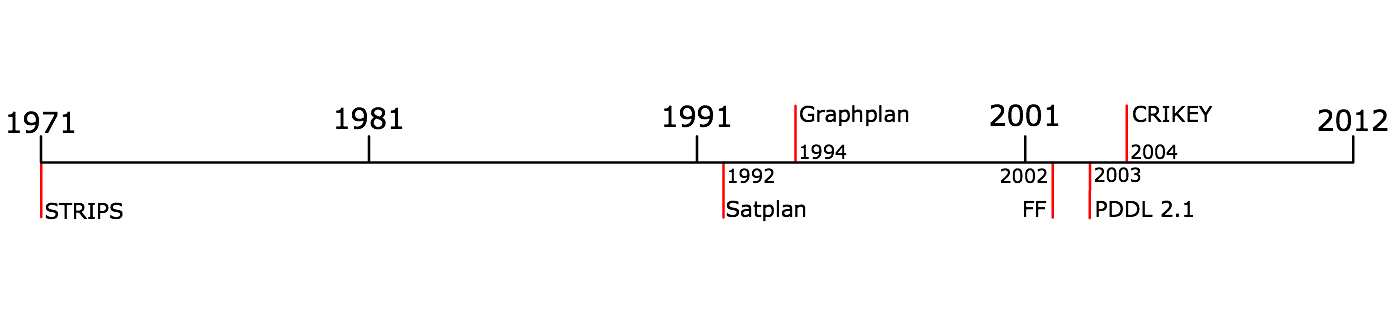
\includegraphics[width=\textwidth]{../images/fig_timeline.jpg}

    \begin{itemize}
		\item (1971) STRIPS (\emph{STranford Research Institute Problem Solver}) (RICHARD E.);
		\item (1992) \emph{Satplan} (A. HENRY);
		\item (1994) \emph{Graphplan} (L. AVRIM);
		\item (2002) FF (\emph{Fast-Forward}) (J. HOFFMANN);
		\item (2003) PDDL 2.1 \emph{Planning Domain Definition Language} (F. MARIA);
		\item (2004) \emph{CRIKEY} (H. KEITH);
    \end{itemize}
\end{frame}

\begin{frame}
    \frametitle{[Planejamento em Intelig�ncia Artificial}
    \begin{itemize}
		\item resolu��o de problemas do mundo real;
		\item planejamento:
		\begin{itemize}
			\item defini-se um estado inicial conhecido;
			\item defini-se um estado final desejado;
			\item busca-se por um conjunto de a��es que leve do inicial ao final;
		\end{itemize}
		\item problema de planejamento:
		\begin{itemize}
			\item encontrar uma sequ�ncia de a��es que, quando executada em um contexto que satisfa�a um estado inicial, vai atingir o objetivo;
		\end{itemize}
		\item plano:
		\begin{itemize}
			\item sequ�ncia de a��es que levam do estado inicial ao estado final;
		\end{itemize}
		\item PDDL:
		\begin{itemize}
			\item interface padr�o para utiliza��o de planejadores;
		\end{itemize}
		\item planejador CRIKEY:
		\begin{itemize}
			\item implementa��o em Java;
			\item heur�stica FF;
		\end{itemize}
    \end{itemize}
\end{frame}
\section[Ambiente Distribu�do]{Ambiente Distribu�do}

\begin{frame}
    \frametitle{Aplica��es \emph{Peer to Peer} (P2P) e \emph{PeerUnit}}
    \begin{itemize}
		\item aplica��es \emph{Peer to Peer} (P2P):
		\begin{itemize}
			\item motiva��o: ser um sistema independente do ambiente de execu��o (grades ou nuvens);
			%\item n�s interconectados capazes de se auto-organizar com objetivo de compartilhar recursos;
		\end{itemize}
		\item \emph{PeerUnit}:
		\begin{itemize}
			\item concebido para realiza��o de testes para sistemas P2P;
			\item cada n� recebe um c�digo pr�-definido em Java;
			\item no c�digo s�o definidos instru��es de como os elementos devem se comportar:
			\begin{itemize}
				\item ordem de execu��o;
				\item tempo limite de execu��o;
				\item quais n�s devem executar.
			\end{itemize}
			\item � um sistema escal�vel;
		\end{itemize}
		\item modifica��es no \emph{PeerUnit}:
		\begin{itemize}
			\item identifica��o �nica para os n�s;
			\item acoplamento do coletor de dados;
			\item adapta��o para execu��o de opera��es;
			\item limita��o de tempo flex�vel;
		\end{itemize}
    \end{itemize}
\end{frame}
\section[Modelo Proposto - Smart Workflow Execution by Planning (SWEP)]{Modelo Proposto - Smart Workflow Execution by Planing (SWEP)}

\begin{frame}
    \frametitle{Proposta SWEP - \emph{Smart Workflow Execution by Planing}}
	\begin{itemize}
		\item Planejador (\emph{CRIKEY});
		\item Ambiente P2P (\emph{PeerUnit});
		\item Caracter�sticas:
		\begin{itemize}
			\item m�tricas flex�veis;
			\item t�cnicas de paraleliza��o;
			\item proveni�ncia e metadados;
		\end{itemize}
	\end{itemize}
\end{frame}

\begin{frame}
    \frametitle{Modelo Proposto - SWEP (\emph{Smart Workflow Execution by Planing})}
	\begin{itemize}
		\item vis�o geral;
		\item vis�o detalhada;
		\item paralelismos;
		\item m�tricas flex�veis;
		\item m�todo de tradu��o;
	\end{itemize}
\end{frame}

\begin{frame}
	\begin{changemargin}{-1cm}{-1cm}
	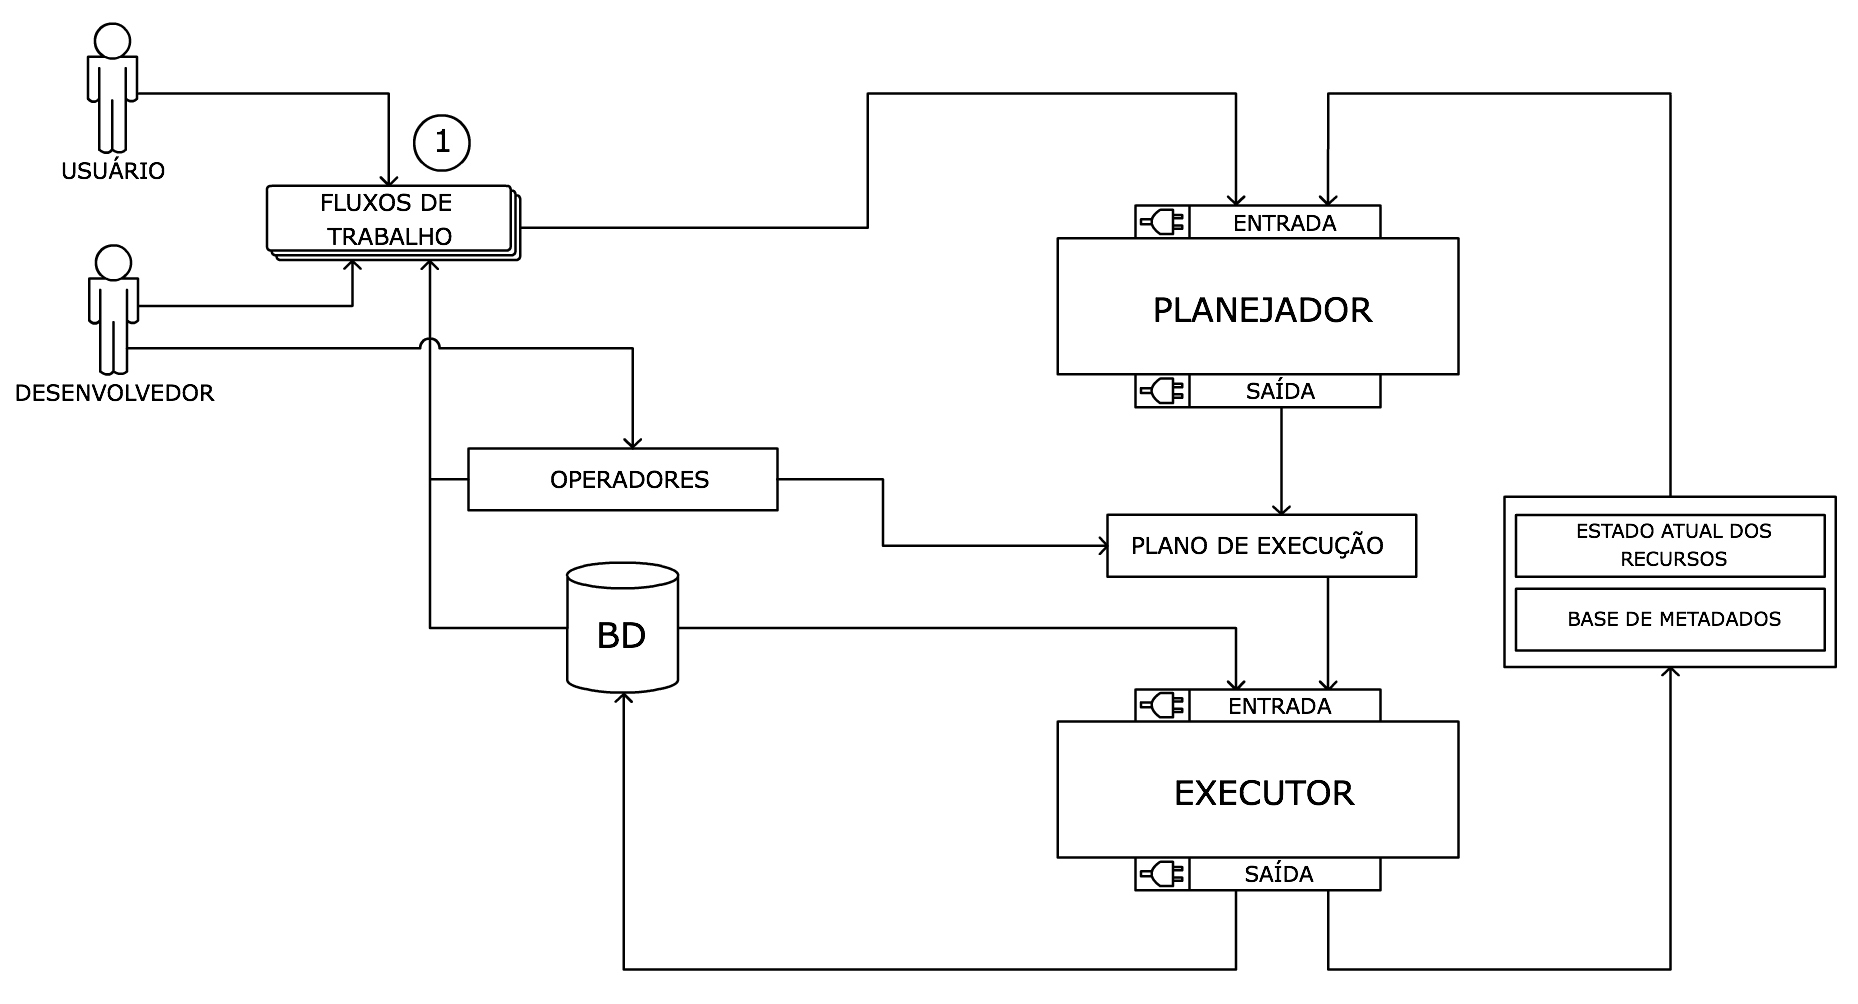
\includegraphics[width=12.8cm]{../images/fig_sys_overview-1.jpg}
	\end{changemargin}
\end{frame}

\begin{frame}
	\begin{changemargin}{-1cm}{-1cm}
	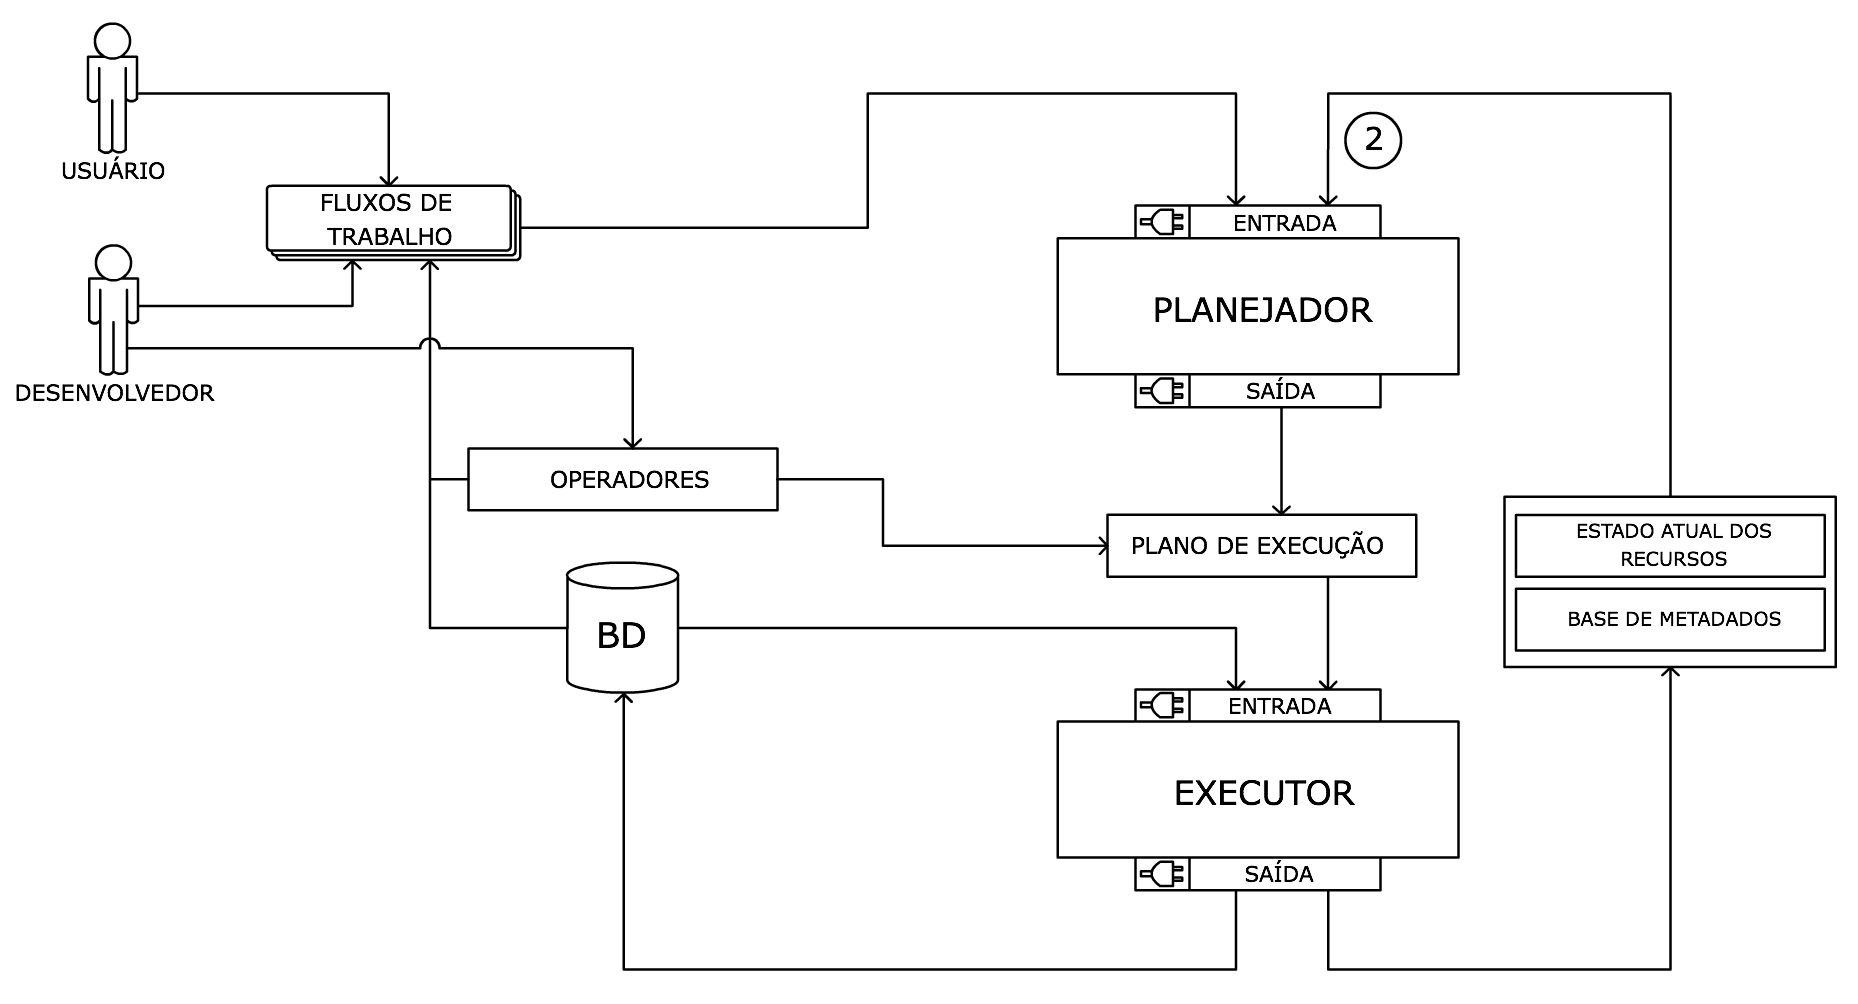
\includegraphics[width=12.8cm]{../images/fig_sys_overview-2.jpg}
	\end{changemargin}
\end{frame}

\begin{frame}
	\begin{changemargin}{-1cm}{-1cm}
	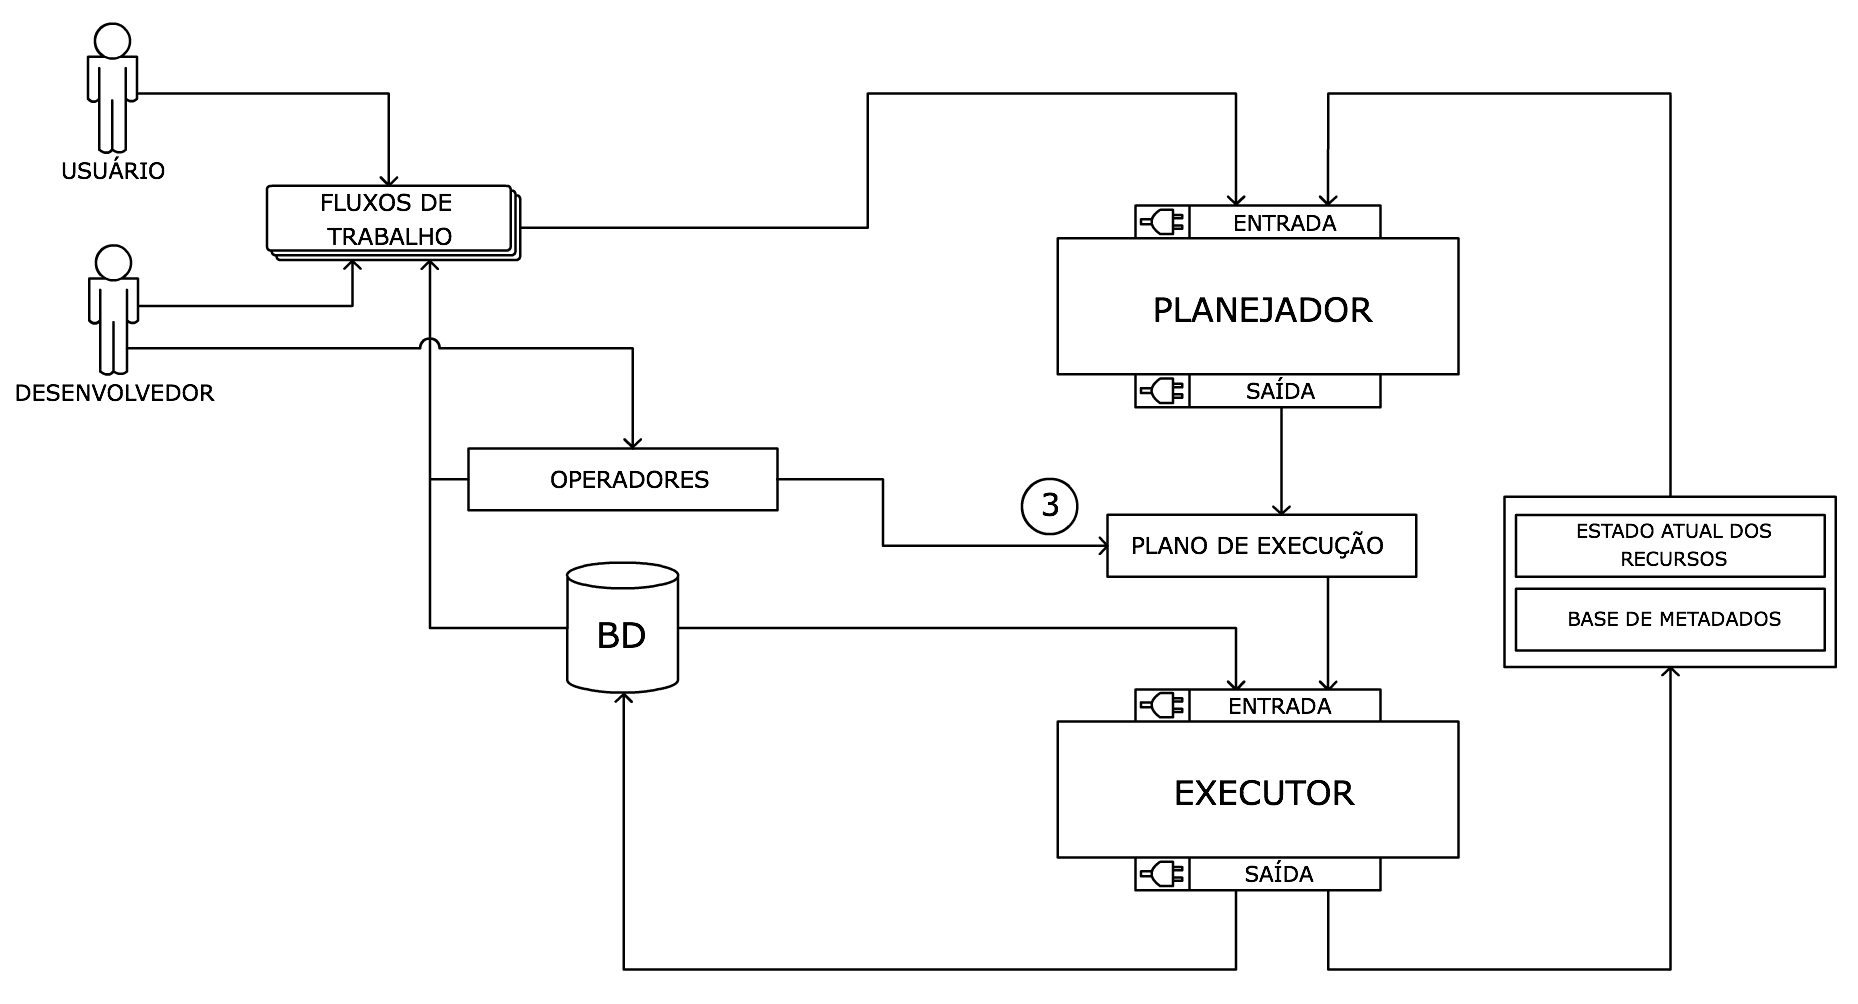
\includegraphics[width=12.8cm]{../images/fig_sys_overview-3.jpg}
	\end{changemargin}
\end{frame}

\begin{frame}
	\begin{changemargin}{-1cm}{-1cm}
	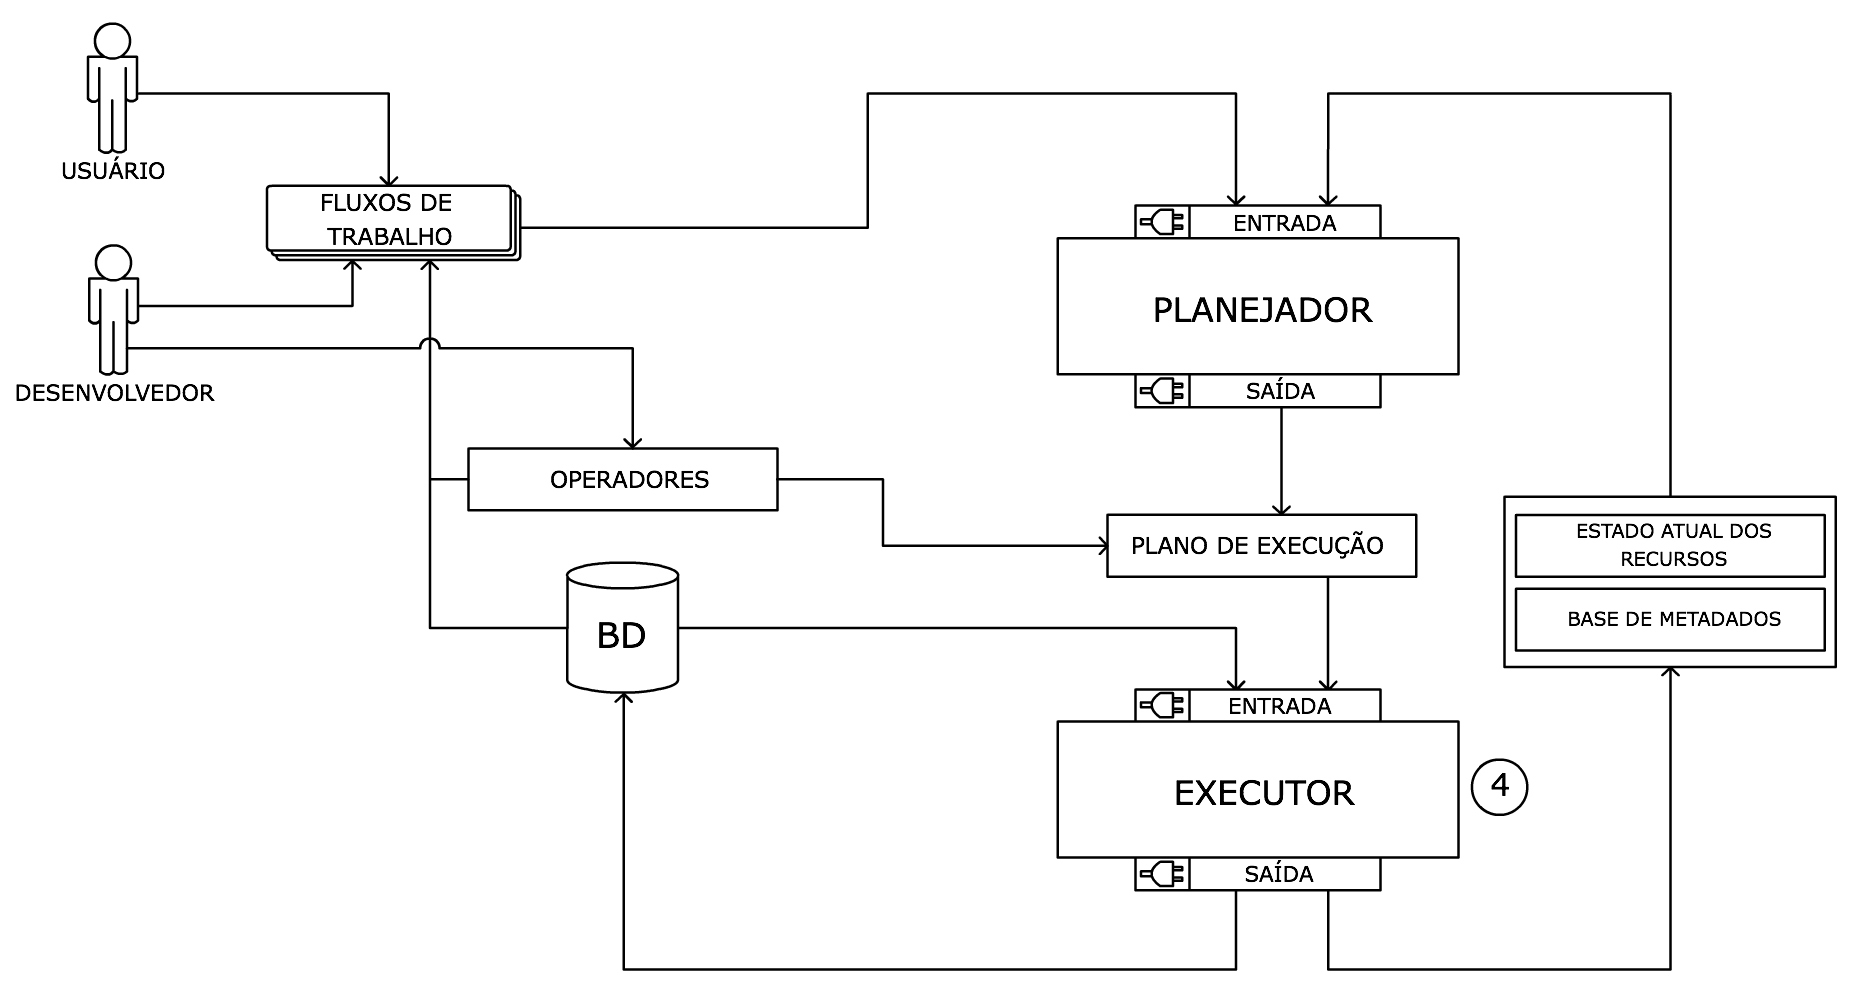
\includegraphics[width=12.8cm]{../images/fig_sys_overview-4.jpg}
	\end{changemargin}
\end{frame}

\begin{frame}
	\begin{changemargin}{-1cm}{-1cm}
	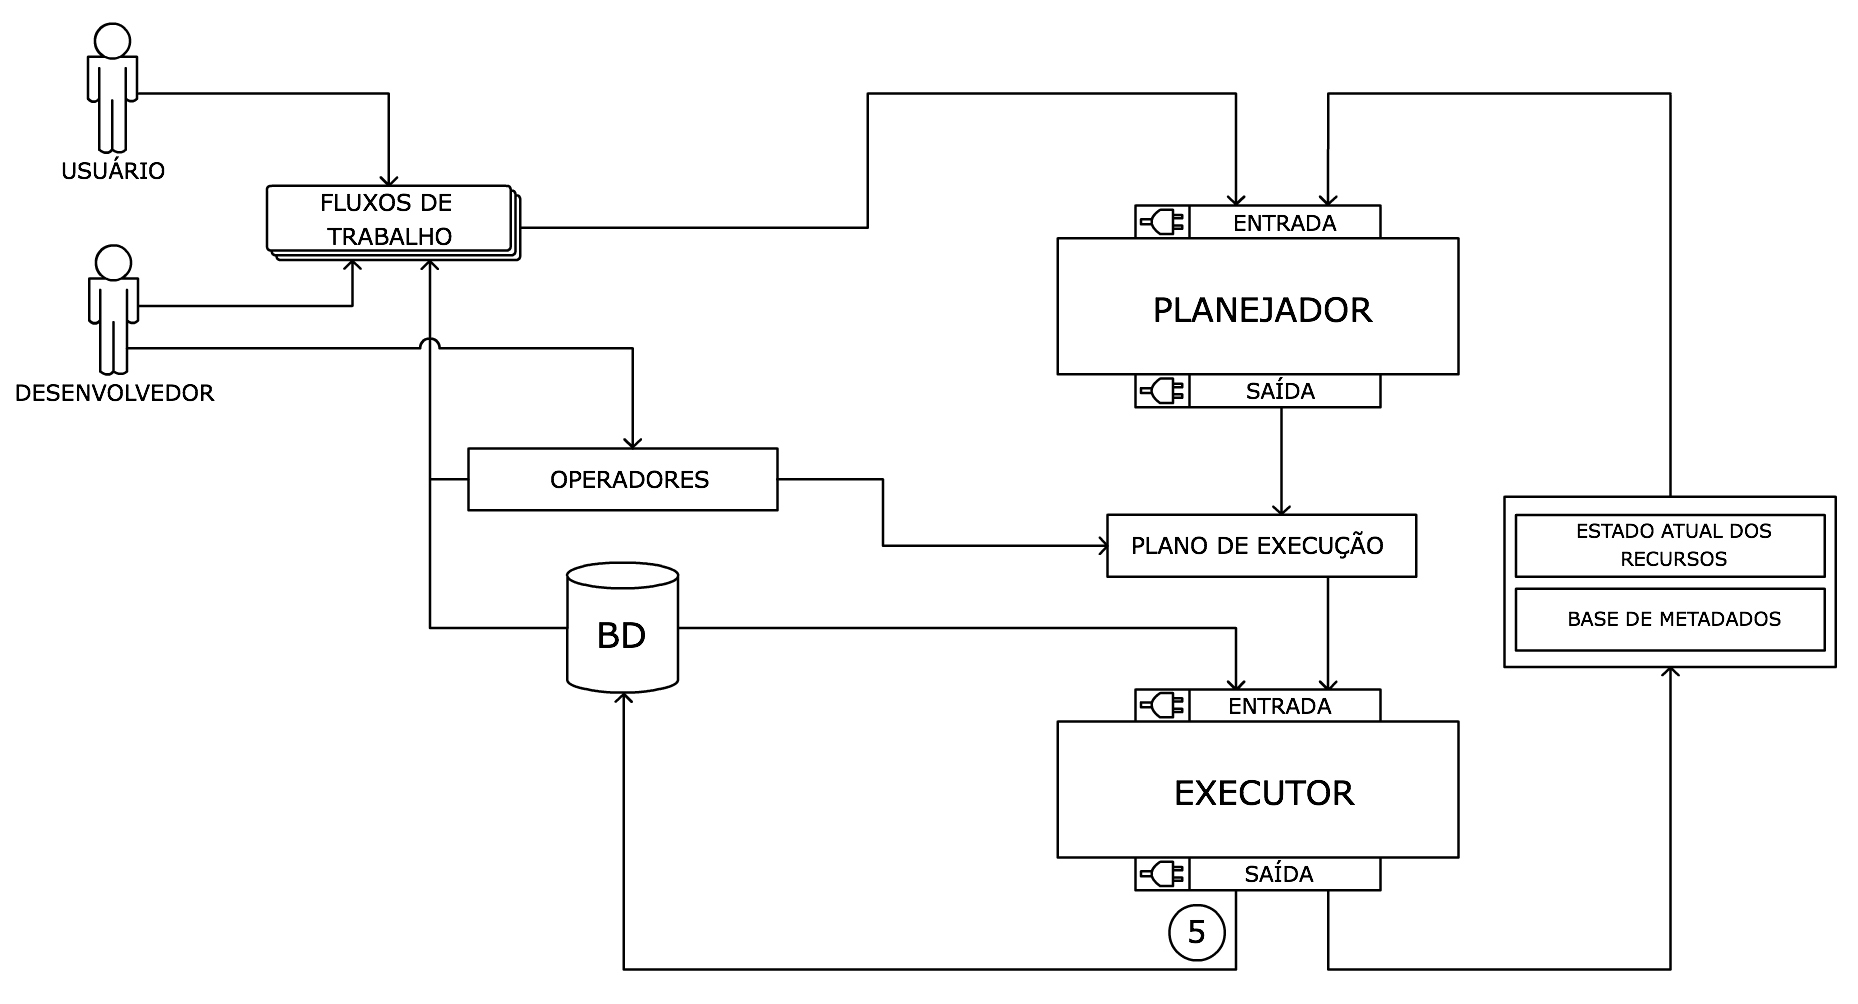
\includegraphics[width=12.8cm]{../images/fig_sys_overview-5.jpg}
	\end{changemargin}
\end{frame}

\begin{frame}
	\begin{changemargin}{-1cm}{-1cm}
	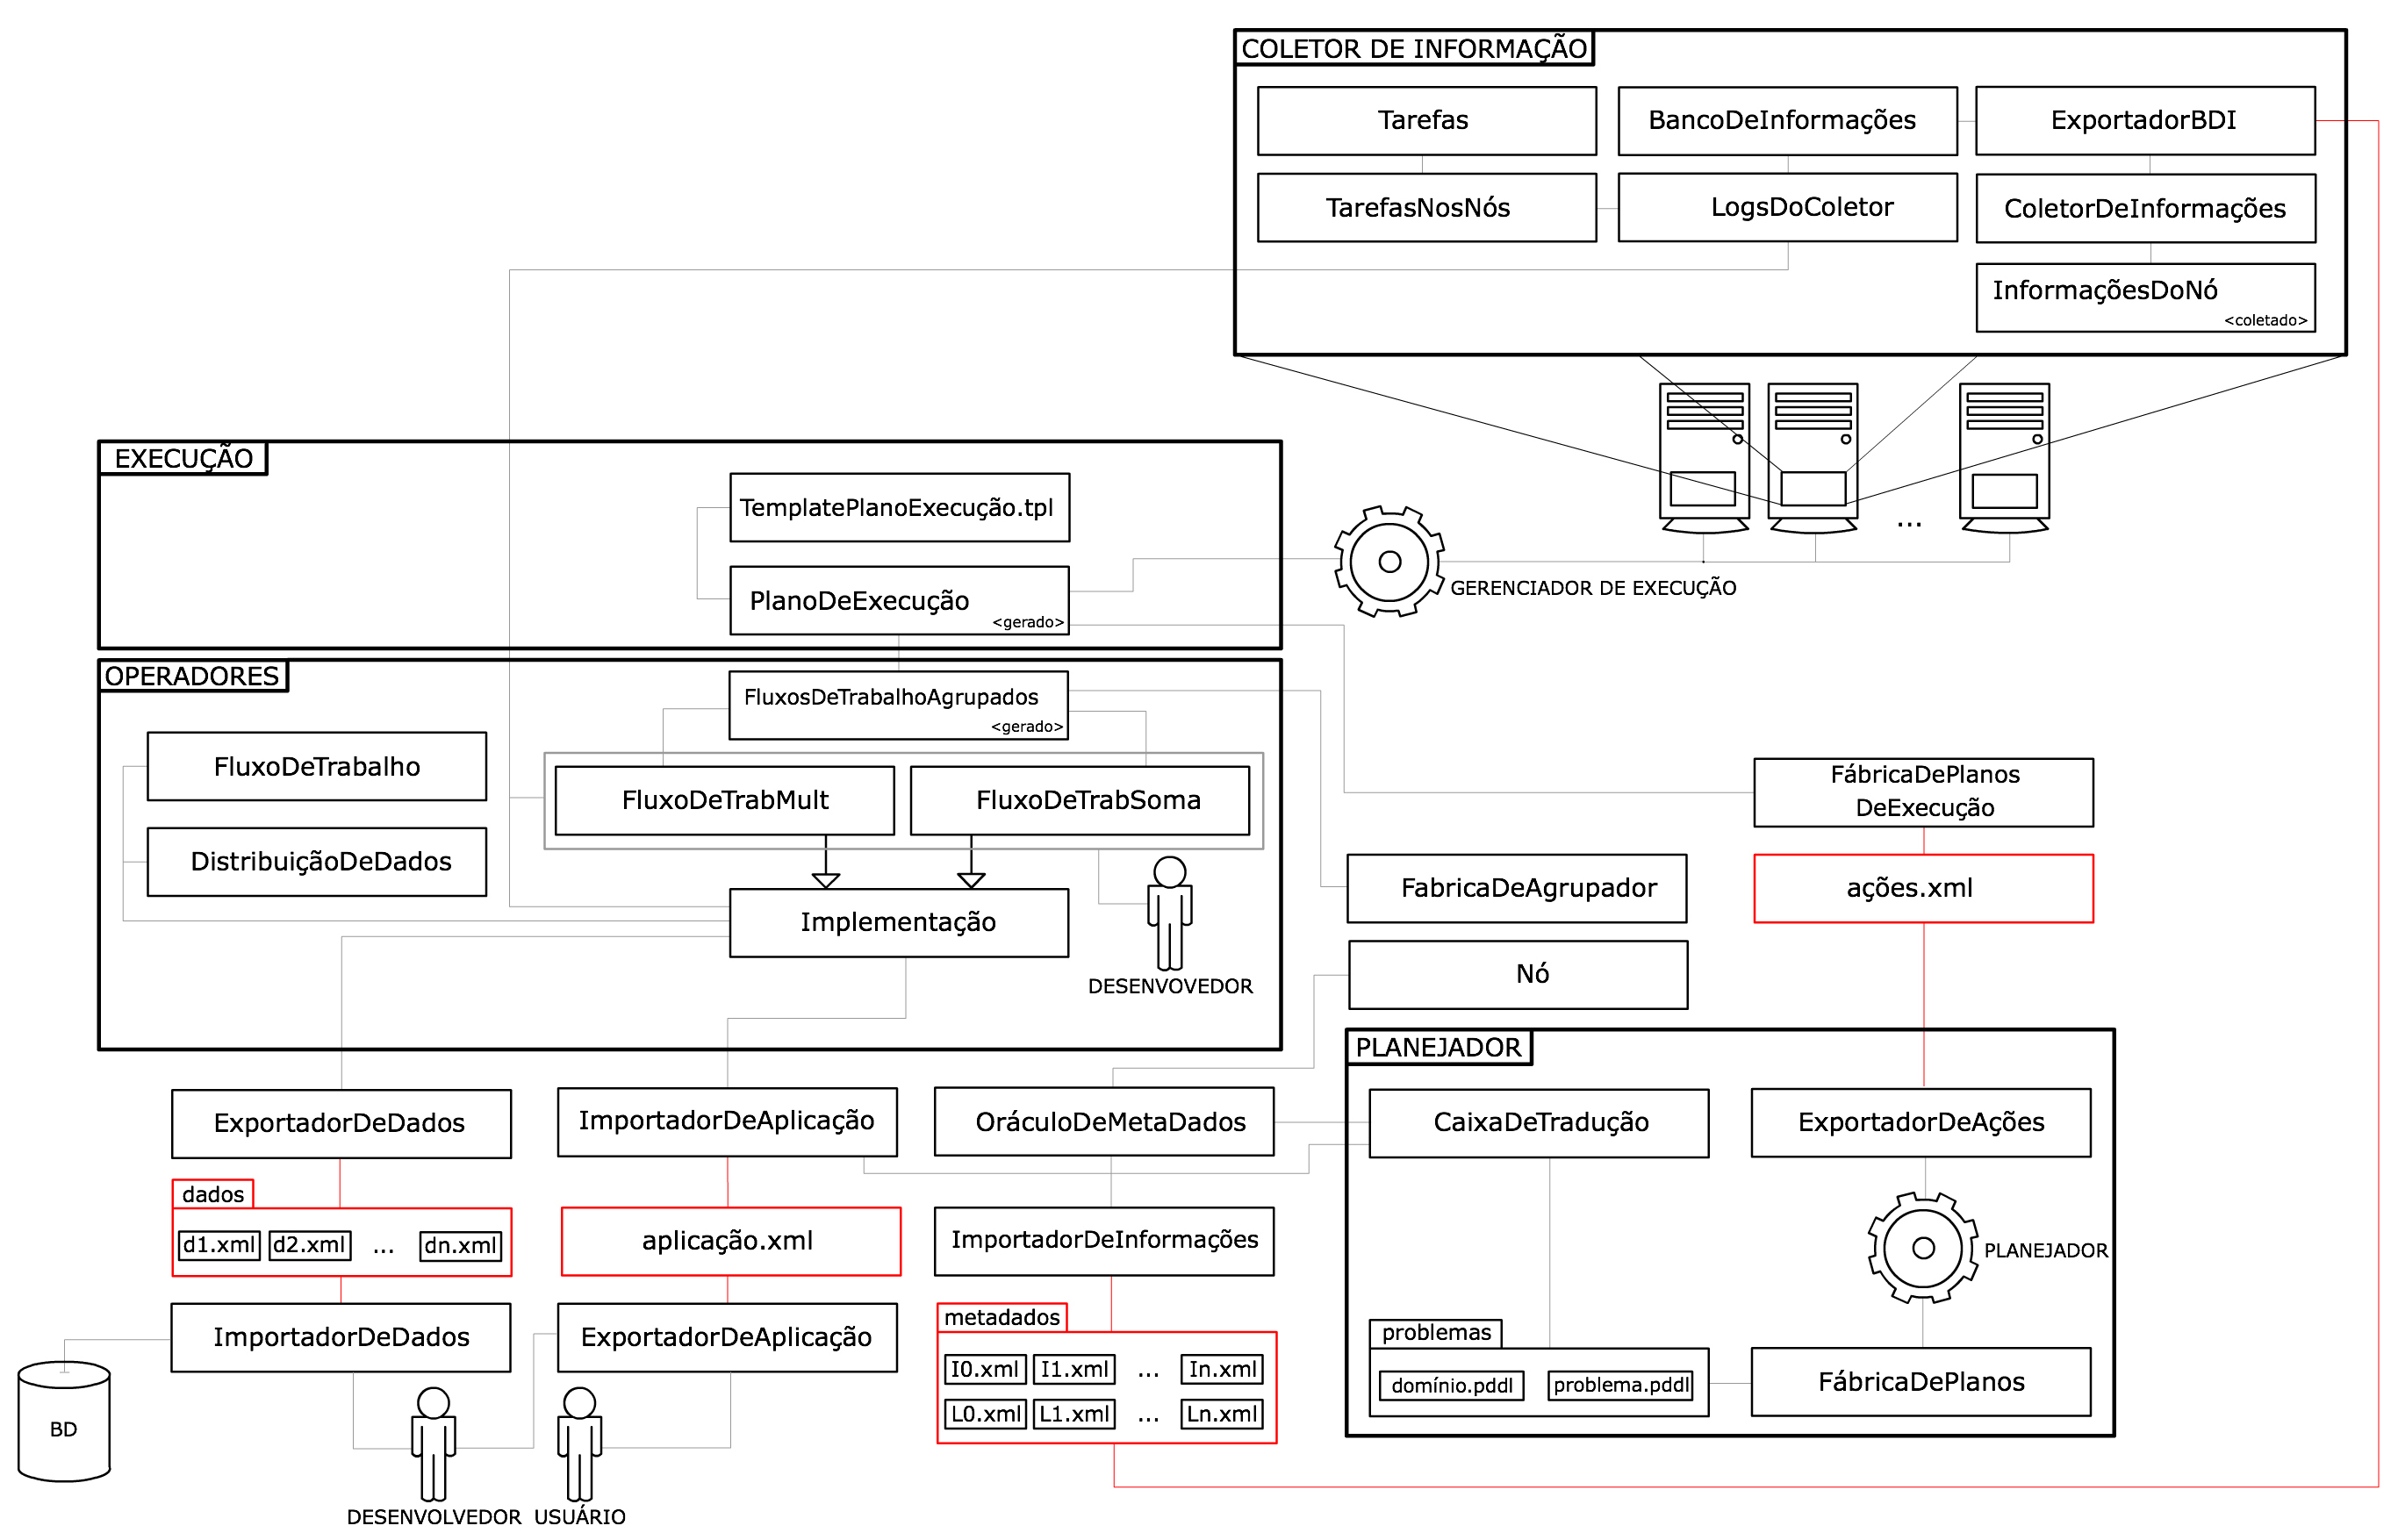
\includegraphics[width=12.8cm]{../images/fig_sys_detailed_red.jpg}
	\end{changemargin}
\end{frame}


\begin{frame}
    \frametitle{Paralelismos}
    \begin{itemize}
		\item paralelismo sobre dados:
		\begin{itemize}
			\item divis�o do processamento de um �nico fluxo de trabalho;
			\item desenvolvedor insere as configura��es (n�mero de n�s ou tamanho dos blocos);
		\end{itemize}
		\item paralelismo sobre execu��o:
		\begin{itemize}
			\item paralelismo entre execu��o de m�ltiplos fluxos de trabalho;
			\item plano paralelo: pondera as depend�ncias de dados;
			\item ordem correta de execu��o;
		\end{itemize}
	\end{itemize}
\end{frame}

\begin{frame}
    \frametitle{Exemplos de Paralelismo - Plano de Execu��o}
	\begin{center}
	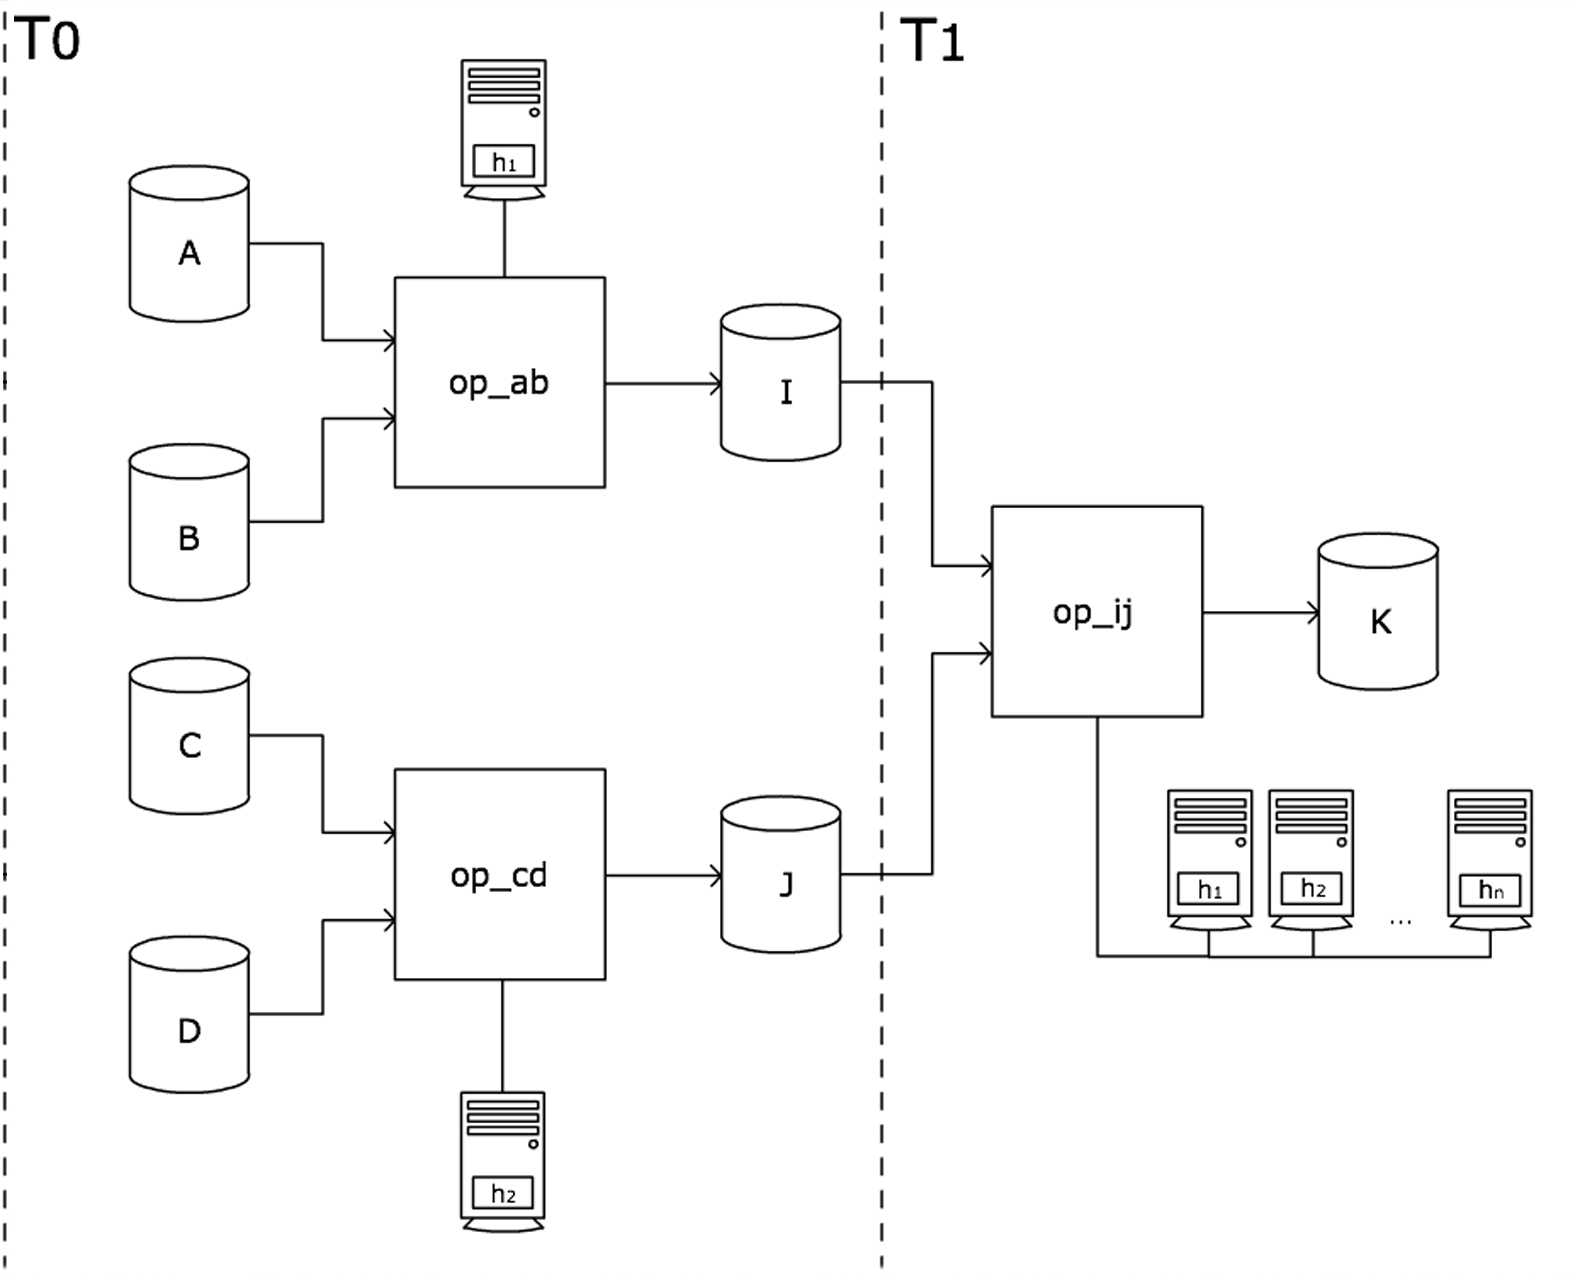
\includegraphics[width=9cm]{../images/fig_sys_parallel_model.jpg}
	\end{center}
\end{frame}

\begin{frame}
    \frametitle{M�trica Flex�vel}
    \begin{itemize}
		\item planejamento baseado nos custos das a��es;
		\item or�culo:
		\begin{itemize}
			\item verifica-se a taxa de ocupa��o dos n�s (livre, parcialmente ocupado ou ocupado);
			\item aplica-se custos pr�-definidos para cada uma das situa��es;
		\end{itemize}
		\item utiliza��o do planejamento de custos para aplica��o de outras m�tricas:
		\begin{itemize}
			\item minimiza��o do consumo de energia el�trica;
			\item maximiza��o de aproveitamento dos recursos;
		\end{itemize}
		\item quantidade de trabalho pode variar de acordo com a situa��o dos recursos, em planos diferentes;
	\end{itemize}
\end{frame}
\chapter{Experimentos}
\label{experimentos}

Neste cap�tulo apresentam-se os experimentos realizados no sistema desenvolvido. A se��o \ref{ex1} mostra um experimento que demonstra a t�cnica de paraleliza��o direta. Na se��o \ref{ex2} apresenta-se um experimento para avalia��o do comportamento utilizando v�rios encadeamentos no fluxo de trabalho. Na se��o \ref{ex3} apresenta-se uma abordagem que demonstra a implementa��o de um operador que trabalha com m�ltiplas entradas e sa�das. Na se��o \ref{ex-consideracoes} faz-se uma analise dos resultados obtidos.

\vspace{1.5cm}

O principal objetivo na an�lise dos resultados est� na corretude dos experimentos bem como a qualidade dos planos gerados. Para os experimentos \ref{ex1} e \ref{ex3} utilizou-se um ambiente de execu��o local no qual simulou-se um ambiente distribu�do. Desta forma, possibilitou-se a reprodu��o dos experimentos com n�s emulados na mesma m�quina. O experimento \ref{ex2} foi um teste para a valida��o do modelo, executado em um ambiente distribu�do com 4 n�s.

A m�quina utilizada para execu��o local possui um processador 2.66 GHz Intel Core 2 Duo com 4GB de mem�ria. As m�quinas do ambiente distribu�do possuem um AMD Opteron com 2.4 GHz e 2GB de mem�ria.

Os testes utilizaram como base os dados extra�dos de matrizes. A motiva��o para a utiliza��o de matrizes � a necessidade de c�lculos simples sobre um grande volume de dados cient�ficos. Para a valida��o do experimento foram utilizadas matrizes quadradas preenchidas por n�meros aleat�rios. Dois operadores foram implementados: soma e multiplica��o de matrizes.

Nas figuras dispostas nesse cap�tulo, cada quadrado representa um operador. Cada operador possui uma identifica��o dos dados que s�o trabalhados. Por exemplo, \emph{op\_a\_b} significa que o operador est� trabalhando com os dados $A$ e $B$. Dentro do quadrado, descreve-se ainda uma informa��o que mostra qual a opera��o efetuada com os dados em quest�o. Por exemplo, \emph{SUM} para soma ou \emph{MULT} para multiplica��o. Os dados s�o representados por cilindros, cada conjunto de dados representa uma matriz e sua identifica��o se d� por letras em mai�sculo. As setas indicam o fluxo dos dados.

Nas tabelas est�o apresentados os resumos de execu��o dos fluxos de trabalho, bem como o plano gerado pelo planejador. A coluna ordem, define a sequencia de execu��o de uma a��o no plano de execu��o. Se uma mesma ordem � repetida em mais de um linha, significa que as a��es ocorrerem em paralelo. A coluna n�, indica qual o n� selecionado para a execu��o da a��o. Se a c�lula apresenta o caractere $*$, significa que a a��o foi executada por todos os n�s. 

Ainda � poss�vel que um subconjunto espec�fico de n�s execute uma a��o, nesse caso suas identifica��es est�o separadas por v�rgula. A coluna operador indica qual o operador utilizado. Se o operador � identificado como \emph{difundir} ent�o h� uma barreira para a publica��o das informa��es, geradas at� o momento, para todos os outros n�s. A coluna dados, indica os dados utilizados para a aplica��o do operador. Quando um dado est� na mesma linha que possui um operador difundir, esse dado � o que ser� publicado para todo o conjunto de n�s. A coluna tempo indica o tempo de execu��o de cada uma das a��es em \UFPRsigla{ms}. As �ltimas linhas mostram um resumo do tempo de execu��o de cada etapa: planejamento, tradu��o, difus�o e processamento. A �ltima linha mostra o tempo total de execu��o.

\section{Experimento 1 - Paraleliza��o Direta}
\label{ex1}

A representa��o do esquema de execu��o dos fluxos de trabalho est�o dispostos na figura \ref{fig:ex1}.

\begin{figure}[ht]
    \centering
    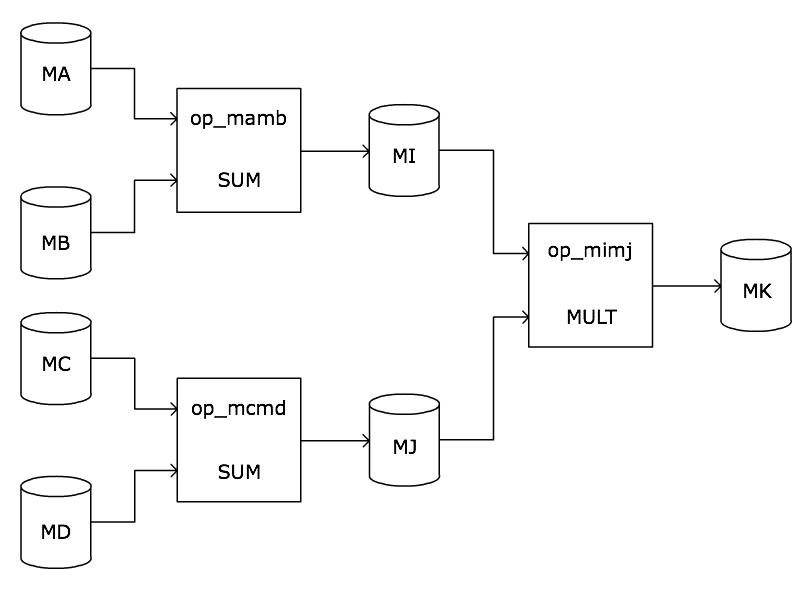
\includegraphics[width=11cm]{images/fig_ex1.jpg}
    \caption{Experimento com opera��es entre matrizes}
    \label{fig:ex1}
\end{figure}

No exemplo s�o definidas tr�s operadores: $op_{\{ma,mb\}}$, $op_{\{mc,md\}}$ e $op_{\{mi,mj\}}$. O operador $op_{\{ma,mb\}}$ espera como entrada os dados $MA$ e $MB$ e gera como sa�da $MI$. J� $op_{\{mc,md\}}$ espera como entrada $MC$ e $MD$ e gera como sa�da $MJ$. O operador $op_{\{mi,mj\}}$ espera como entrada $MI$ e $MJ$ e gera como sa�da $MK$, que em nosso exemplo � o objetivo. A defini��o do arquivo que cont�m a descri��o dos fluxos de trabalho est� transcrita no ap�ndice \ref{ap-aplicacao}.

Foram utilizados dois n�s para a execu��o do experimento: $h_0$ e $h_1$. Neste experimento, analisa-se os modelos paralelos abordados no cap�tulo \ref{modelo}. A \emph{paraleliza��o direta} (se��o \ref{par-direta}) e o \emph{paralelismo sobre execu��o} (se��o \ref{paralelismo-execucao}). A figura \ref{fig:ex1_parallel} mostra a distribui��o das tarefas e os respectivos n�s utilizados para execu��o.

\begin{figure}[ht]
    \centering
    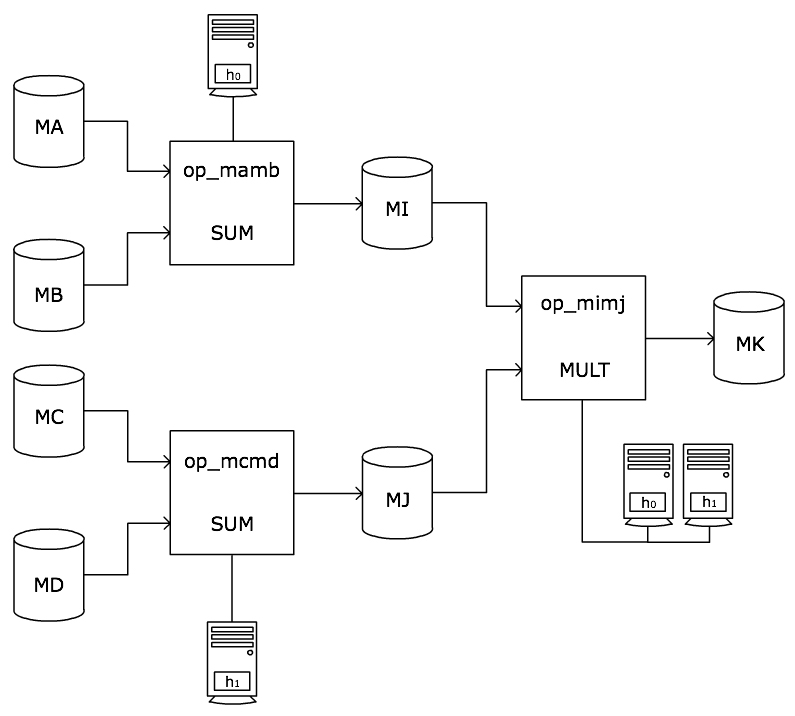
\includegraphics[width=11cm]{images/fig_ex1_parallel.jpg}
    \caption{Diagrama do experimento 1}
    \label{fig:ex1_parallel}
\end{figure}

A paraleliza��o direta ocorre na execu��o distribu�da do operador $op_{\{mi,mj\}}$. O paralelismo sobre execu��o est� exemplificado na execu��o simult�nea de $op_{\{ma,mb\}}$ e $op_{\{mc,md\}}$.

A tabela \ref{tab:ex1} detalha as informa��es extra�das do experimento.

\begin{table}[ht]
	\centering
	\caption{Resultados do experimento com paraleliza��o direta}
	\label{tab:ex1}
	\begin{tabular}{|l|l|l|l|l|}
	\hline
	\multicolumn{1}{|c|}{Ordem} & \multicolumn{1}{c|}{Host} & \multicolumn{1}{c|}{Operador} & \multicolumn{1}{c|}{Dados} & \multicolumn{1}{c|}{Tempo (ms)} \\ 
	\hline
	\multicolumn{1}{|c|}{1} & \multicolumn{1}{c|}{$h_0$} & \multicolumn{1}{c|}{SUM} & \multicolumn{1}{c|}{$MA,MB$} & \multicolumn{1}{r|}{4779} \\ 
	\hline
	\multicolumn{1}{|c|}{1} & \multicolumn{1}{c|}{$h_1$} & \multicolumn{1}{c|}{SUM} & \multicolumn{1}{c|}{$MC,MD$} & \multicolumn{1}{r|}{3935} \\ 
	\hline
	\multicolumn{1}{|c|}{2} & \multicolumn{1}{c|}{*} & \multicolumn{1}{c|}{DIFUNDIR} & \multicolumn{1}{c|}{$MI$} & \multicolumn{1}{r|}{5617} \\ 
	\hline
	\multicolumn{1}{|c|}{2} & \multicolumn{1}{c|}{*} & \multicolumn{1}{c|}{DIFUNDIR} & \multicolumn{1}{c|}{$MJ$} & \multicolumn{1}{r|}{4203} \\ 
	\hline
	\multicolumn{1}{|c|}{3} & \multicolumn{1}{c|}{$h_0, h_1$} & \multicolumn{1}{c|}{MULT} & \multicolumn{1}{c|}{$MI,MJ$} & \multicolumn{1}{r|}{3170} \\ 
	\hline
	\multicolumn{1}{|c|}{4} & \multicolumn{1}{c|}{*} & \multicolumn{1}{c|}{DIFUNDIR} & \multicolumn{1}{c|}{$MK$} & \multicolumn{1}{r|}{2880} \\ 
	\hline
	\multicolumn{1}{|c|}{5} & \multicolumn{1}{c|}{*} & \multicolumn{1}{c|}{coletor de informa��o} & \multicolumn{1}{c|}{metadados} & \multicolumn{1}{r|}{31} \\ 
	\hline
	\multicolumn{4}{|c|}{tempo de planejamento} & \multicolumn{1}{r|}{1014} \\ 
	\hline
	\multicolumn{4}{|c|}{tempo de tradu��o} & \multicolumn{1}{r|}{523} \\ 
	\hline
	\multicolumn{4}{|c|}{tempo de difus�o} & \multicolumn{1}{r|}{12700} \\ 
	\hline
	\multicolumn{4}{|c|}{tempo processamento} & \multicolumn{1}{r|}{11935} \\ 
	\hline
	\multicolumn{4}{|c|}{tempo total} & \multicolumn{1}{r|}{26172} \\ 
	\hline
	\end{tabular}
\end{table}

Nota-se que o planejador considerou a execu��o simult�nea dos operadores $op_{\{ma,mb\}}$ e $op_{\{mc,md\}}$ na etapa $1$, pois os operadores n�o possuem qualquer depend�ncia de dados. O tempo para execu��o da opera��o de soma foi semelhante, para o operador $op_{\{ma,mb\}}$ gastou-se $4779$ms, enquanto que o operador $op_{\{mc,md\}}$ terminou a execu��o em $3935$ms. 

Nas etapas $2$ e $4$ nota-se a opera��o de difus�o. Essa opera��o distribui os resultados obtidos pelos operadores para todos os outros n�s do ambiente, visto que algum operador seguinte pode utilizar os dados gerados na opera��o em quest�o.

A etapa $3$ utiliza dois n�s para a execu��o da opera��o de multiplica��o. O tipo de paraleliza��o adotada � direta, por isso, o desenvolvedor informa os par�metros para a execu��o paralela dos dados. Ambos os n�s dispon�veis foram escolhidos para a divis�o dos dados, e a opera��o completa levou $3170$ms.

\section{Experimento 2 - Encadeamento de Fluxos de Trabalho}
\label{ex2}

A representa��o do esquema de execu��o do fluxo de trabalho est� disposta na figura \ref{fig:ex2}.

\begin{landscape}
	
\begin{figure}[ht]
    \centering
    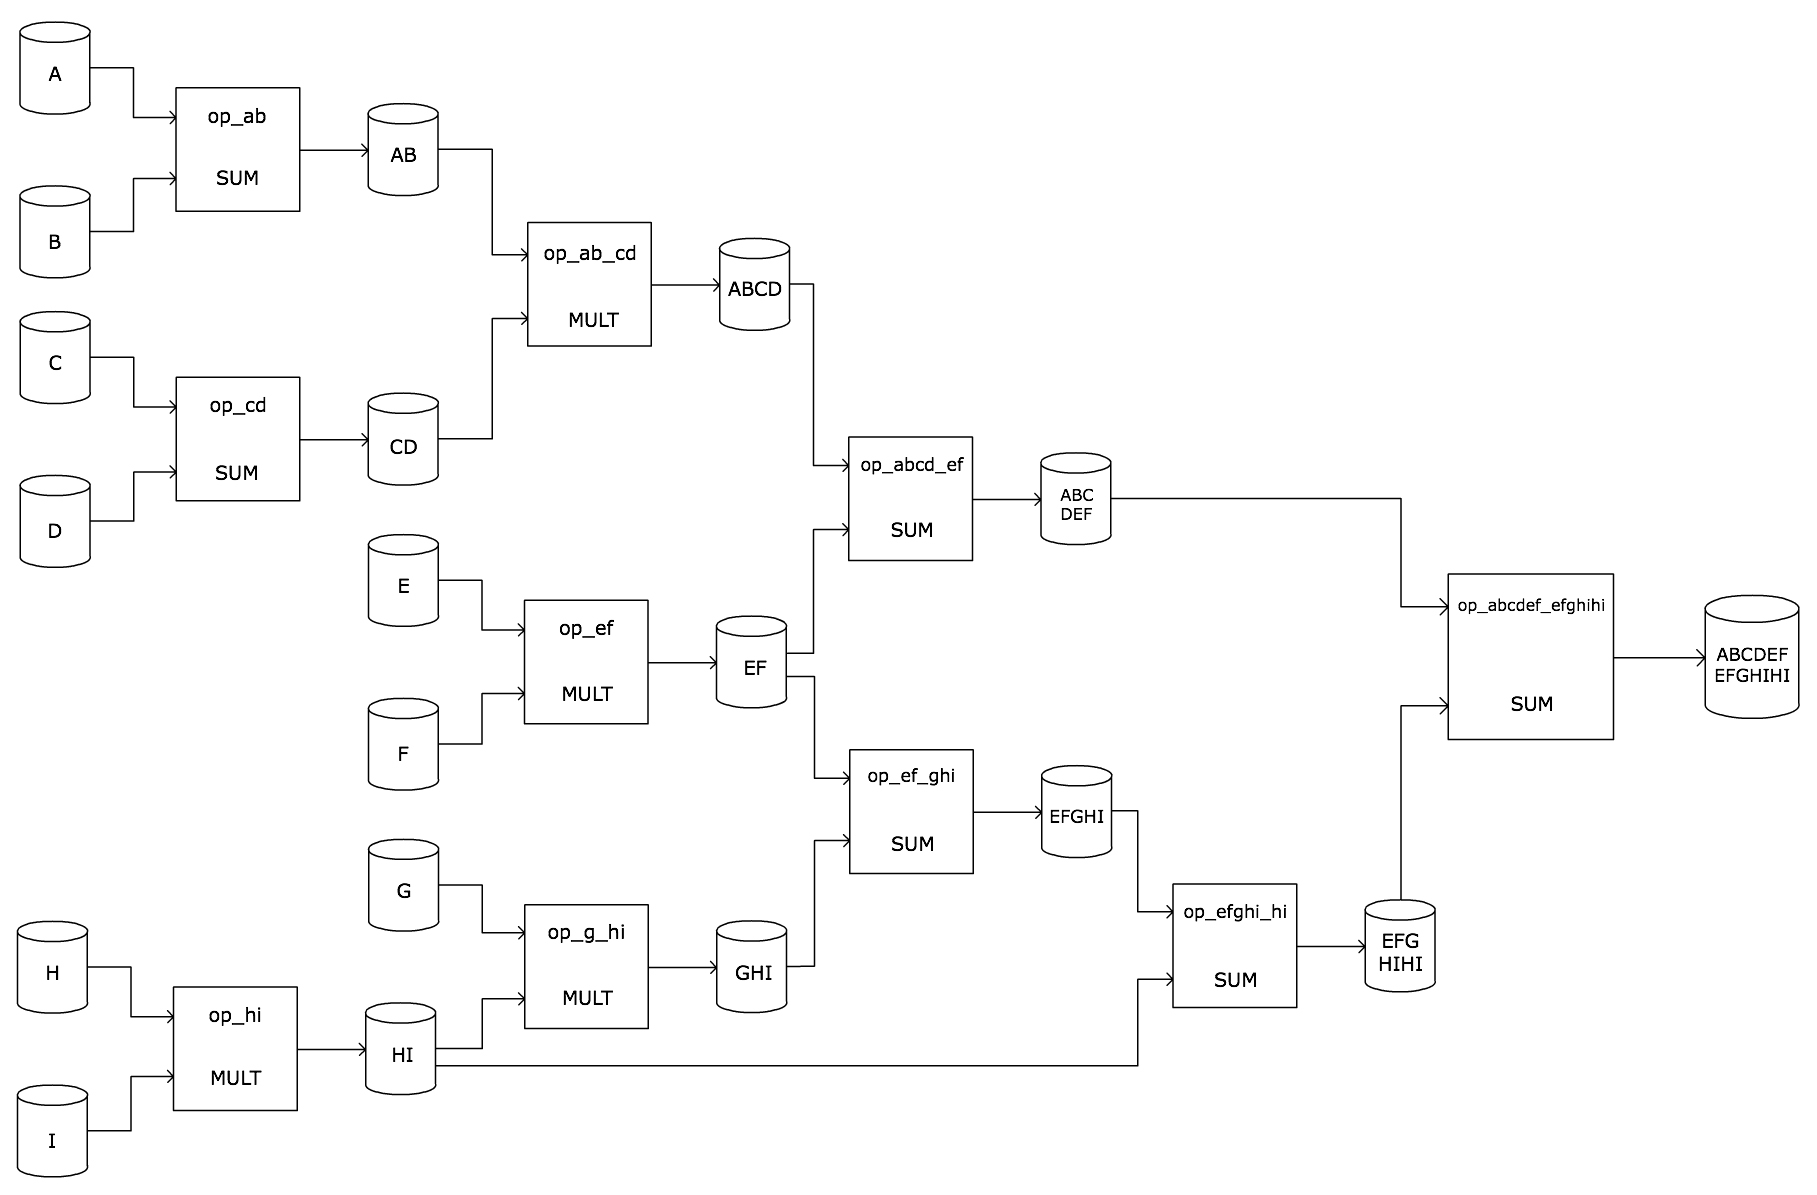
\includegraphics[width=22cm]{images/fig_ex2.jpg}
    \caption{Diagrama do experimento 2}
    \label{fig:ex2}
\end{figure}

\end{landscape}

No exemplo s�o definidos dez operadores: $op_{\{a,b\}}$, $op_{\{c,d\}}$, $op_{\{h,i\}}$, $ op_{\{e,f\}}$, $op_{\{ab,cd\}}$, $op_{\{g,hi\}}$, $op_{\{abcd,ef\}}$, $op_{\{ef,ghi\}}$, $op_{\{efghi_hi\}}$ e $op_{\{abcdef,efghihi\}}$. A indexa��o de cada operador define sua entrada de dados. O objetivo do experimento � a obten��o do dado final $ABCDEFEFGHIHI$.

Para o experimento foram utilizados 4 n�s: $h_0, h_1, h_2$ e $h_3$. Testou-se a validade do componente \emph{Or�culoDeMetaDados} que retorna a taxa de ocupa��o dos n�s dispon�veis, em tr�s situa��es diferentes:

\begin{enumerate}
	\item quatro n�s dispon�veis;
	\item dois n�s dispon�veis ($h_0$ e $h_1$) e dois n�s parcialmente dispon�veis ($h_2$ e $h_3$);
	\item um n� dispon�vel ($h_0$) e tr�s parcialmente dispon�veis ($h_1$, $h_2$ e $h_3$).
\end{enumerate}

As tabelas \ref{tab:ex2a}, \ref{tab:ex2b}, \ref{tab:ex2c} demonstram os resultados para as tr�s situa��es, respectivamente.

\newpage

\begin{table}[ht]
	\centering
	\caption{Encadeamento de fluxos - 4 n�s dispon�veis}
	\label{tab:ex2a}
	\begin{tabular}{|l|l|l|l|l|}
	\hline
	\multicolumn{1}{|c|}{Ordem} & \multicolumn{1}{c|}{Host} & \multicolumn{1}{c|}{Operador} & \multicolumn{1}{c|}{Dados} & \multicolumn{1}{c|}{Tempo (ms)} \\ 
	\hline
	\multicolumn{1}{|c|}{1} & \multicolumn{1}{c|}{$h_1$} & \multicolumn{1}{c|}{MULT} & \multicolumn{1}{c|}{$H,I$} & \multicolumn{1}{r|}{17400} \\ 
	\hline
	\multicolumn{1}{|c|}{1} & \multicolumn{1}{c|}{$h_3$} & \multicolumn{1}{c|}{MULT} & \multicolumn{1}{c|}{$E,F$} & \multicolumn{1}{r|}{17160} \\ 
	\hline
	\multicolumn{1}{|c|}{1} & \multicolumn{1}{c|}{$h_0$} & \multicolumn{1}{c|}{SUM} & \multicolumn{1}{c|}{$C,D$} & \multicolumn{1}{r|}{16699} \\ 
	\hline
	\multicolumn{1}{|c|}{1} & \multicolumn{1}{c|}{$h_2$} & \multicolumn{1}{c|}{SUM} & \multicolumn{1}{c|}{$A,B$} & \multicolumn{1}{r|}{17738} \\ 
	\hline
	\multicolumn{1}{|c|}{2} & \multicolumn{1}{c|}{*} & \multicolumn{1}{c|}{DIFUNDIR} & \multicolumn{1}{c|}{$EF$} & \multicolumn{1}{r|}{16616} \\ 
	\hline
	\multicolumn{1}{|c|}{2} & \multicolumn{1}{c|}{*} & \multicolumn{1}{c|}{DIFUNDIR} & \multicolumn{1}{c|}{$HI$} & \multicolumn{1}{r|}{15818} \\ 
	\hline
	\multicolumn{1}{|c|}{2} & \multicolumn{1}{c|}{*} & \multicolumn{1}{c|}{DIFUNDIR} & \multicolumn{1}{c|}{$AB$} & \multicolumn{1}{r|}{14650} \\ 
	\hline
	\multicolumn{1}{|c|}{2} & \multicolumn{1}{c|}{*} & \multicolumn{1}{c|}{DIFUNDIR} & \multicolumn{1}{c|}{$CD$} & \multicolumn{1}{r|}{14472} \\ 
	\hline
	\multicolumn{1}{|c|}{3} & \multicolumn{1}{c|}{$h_2$} & \multicolumn{1}{c|}{MULT} & \multicolumn{1}{c|}{$G,HI$} & \multicolumn{1}{r|}{13168} \\ 
	\hline
	\multicolumn{1}{|c|}{3} & \multicolumn{1}{c|}{$h_0$} & \multicolumn{1}{c|}{MULT} & \multicolumn{1}{c|}{$AB,CD$} & \multicolumn{1}{r|}{14475} \\ 
	\hline
	\multicolumn{1}{|c|}{4} & \multicolumn{1}{c|}{*} & \multicolumn{1}{c|}{DIFUNDIR} & \multicolumn{1}{c|}{$GHI$} & \multicolumn{1}{r|}{14908} \\ 
	\hline
	\multicolumn{1}{|c|}{4} & \multicolumn{1}{c|}{*} & \multicolumn{1}{c|}{DIFUNDIR} & \multicolumn{1}{c|}{$ABCD$} & \multicolumn{1}{r|}{14637} \\ 
	\hline
	\multicolumn{1}{|c|}{5} & \multicolumn{1}{c|}{$h_1$} & \multicolumn{1}{c|}{SUM} & \multicolumn{1}{c|}{$EF,GHI$} & \multicolumn{1}{r|}{14189} \\ 
	\hline
	\multicolumn{1}{|c|}{5} & \multicolumn{1}{c|}{$h_3$} & \multicolumn{1}{c|}{SUM} & \multicolumn{1}{c|}{$ABCD,EF$} & \multicolumn{1}{r|}{13622} \\ 
	\hline
	\multicolumn{1}{|c|}{6} & \multicolumn{1}{c|}{*} & \multicolumn{1}{c|}{DIFUNDIR} & \multicolumn{1}{c|}{$EFGHI$} & \multicolumn{1}{r|}{14661} \\ 
	\hline
	\multicolumn{1}{|c|}{6} & \multicolumn{1}{c|}{*} & \multicolumn{1}{c|}{DIFUNDIR} & \multicolumn{1}{c|}{$ABCDEF$} & \multicolumn{1}{r|}{14881} \\ 
	\hline
	\multicolumn{1}{|c|}{7} & \multicolumn{1}{c|}{$h_3$} & \multicolumn{1}{c|}{SUM} & \multicolumn{1}{c|}{$EFGHI,HI$} & \multicolumn{1}{r|}{13584} \\ 
	\hline
	\multicolumn{1}{|c|}{8} & \multicolumn{1}{c|}{*} & \multicolumn{1}{c|}{DIFUNDIR} & \multicolumn{1}{c|}{$EFGHIHI$} & \multicolumn{1}{r|}{15042} \\ 
	\hline
	\multicolumn{1}{|c|}{9} & \multicolumn{1}{c|}{$h_0$} & \multicolumn{1}{c|}{SUM} & \multicolumn{1}{c|}{$ABCDEF,EFGHIHI$} & \multicolumn{1}{r|}{14900} \\ 
	\hline
	\multicolumn{1}{|c|}{10} & \multicolumn{1}{c|}{*} & \multicolumn{1}{c|}{DIFUNDIR} & \multicolumn{1}{c|}{$ABCDEFEFGHIHI$} & \multicolumn{1}{r|}{15145} \\ 
	\hline
	\multicolumn{1}{|c|}{11} & \multicolumn{1}{c|}{*} & \multicolumn{1}{c|}{coletor de informa��o} & \multicolumn{1}{c|}{metadados} & \multicolumn{1}{r|}{39} \\ 
	\hline
	\multicolumn{4}{|c|}{tempo de planejamento} & \multicolumn{1}{r|}{3523} \\ 
	\hline
	\multicolumn{4}{|c|}{tempo de tradu��o} & \multicolumn{1}{r|}{1301} \\ 
	\hline
	\multicolumn{4}{|c|}{tempo de difus�o} & \multicolumn{1}{r|}{150830} \\ 
	\hline
	\multicolumn{4}{|c|}{tempo processamento} & \multicolumn{1}{r|}{153016} \\ 
	\hline
	\multicolumn{4}{|c|}{tempo total} & \multicolumn{1}{r|}{308670} \\ 
	\hline
	\end{tabular}
\end{table}

Nota-se que com 4 n�s dispon�veis o planejador elabora o plano �timo, distribuindo o m�ximo de operadores poss�vel na etapa $1$. A difus�o dos resultados ocorre nas etapas $2$, $4$, $6$, $8$ e $10$. As etapas �mpares s�o respons�veis pelos c�lculos dos operadores enquanto que as etapas pares s�o respons�veis pela difus�o dos resultados obtidos.

\newpage

\begin{table}[ht]
	\centering
	\caption{Encadeamento de fluxos - 2 n�s dispon�veis e 2 parcialmente dispon�veis}
	\label{tab:ex2b}
	\begin{tabular}{|l|l|l|l|l|}
	\hline
	\multicolumn{1}{|c|}{Ordem} & \multicolumn{1}{c|}{Host} & \multicolumn{1}{c|}{Operador} & \multicolumn{1}{c|}{Dados} & \multicolumn{1}{c|}{Tempo (ms)} \\ 
	\hline
	\multicolumn{1}{|c|}{1} & \multicolumn{1}{c|}{$h_1$} & \multicolumn{1}{c|}{MULT} & \multicolumn{1}{c|}{$H,I$} & \multicolumn{1}{r|}{18999} \\ 
	\hline
	\multicolumn{1}{|c|}{1} & \multicolumn{1}{c|}{$h_0$} & \multicolumn{1}{c|}{SUM} & \multicolumn{1}{c|}{$C,D$} & \multicolumn{1}{r|}{17012} \\ 
	\hline
	\multicolumn{1}{|c|}{1} & \multicolumn{1}{c|}{$h_3$} & \multicolumn{1}{c|}{SUM} & \multicolumn{1}{c|}{$A,B$} & \multicolumn{1}{r|}{17541} \\ 
	\hline
	\multicolumn{1}{|c|}{2} & \multicolumn{1}{c|}{*} & \multicolumn{1}{c|}{DIFUNDIR} & \multicolumn{1}{c|}{$HI$} & \multicolumn{1}{r|}{17243} \\ 
	\hline
	\multicolumn{1}{|c|}{2} & \multicolumn{1}{c|}{*} & \multicolumn{1}{c|}{DIFUNDIR} & \multicolumn{1}{c|}{$CD$} & \multicolumn{1}{r|}{16543} \\ 
	\hline
	\multicolumn{1}{|c|}{2} & \multicolumn{1}{c|}{*} & \multicolumn{1}{c|}{DIFUNDIR} & \multicolumn{1}{c|}{$AB$} & \multicolumn{1}{r|}{15426} \\ 
	\hline
	\multicolumn{1}{|c|}{3} & \multicolumn{1}{c|}{$h_1$} & \multicolumn{1}{c|}{MULT} & \multicolumn{1}{c|}{$E,F$} & \multicolumn{1}{r|}{15188} \\ 
	\hline
	\multicolumn{1}{|c|}{3} & \multicolumn{1}{c|}{$h_0$} & \multicolumn{1}{c|}{MULT} & \multicolumn{1}{c|}{$G,HI$} & \multicolumn{1}{r|}{13453} \\ 
	\hline
	\multicolumn{1}{|c|}{4} & \multicolumn{1}{c|}{*} & \multicolumn{1}{c|}{DIFUNDIR} & \multicolumn{1}{c|}{$EF$} & \multicolumn{1}{r|}{15377} \\ 
	\hline
	\multicolumn{1}{|c|}{4} & \multicolumn{1}{c|}{*} & \multicolumn{1}{c|}{DIFUNDIR} & \multicolumn{1}{c|}{$GHI$} & \multicolumn{1}{r|}{15170} \\ 
	\hline
	\multicolumn{1}{|c|}{5} & \multicolumn{1}{c|}{$h_1$} & \multicolumn{1}{c|}{SUM} & \multicolumn{1}{c|}{$EF,GHI$} & \multicolumn{1}{r|}{15286} \\ 
	\hline
	\multicolumn{1}{|c|}{5} & \multicolumn{1}{c|}{$h_0$} & \multicolumn{1}{c|}{MULT} & \multicolumn{1}{c|}{$AB,CD$} & \multicolumn{1}{r|}{14212} \\ 
	\hline
	\multicolumn{1}{|c|}{6} & \multicolumn{1}{c|}{*} & \multicolumn{1}{c|}{DIFUNDIR} & \multicolumn{1}{c|}{$EFGHI$} & \multicolumn{1}{r|}{15334} \\ 
	\hline
	\multicolumn{1}{|c|}{6} & \multicolumn{1}{c|}{*} & \multicolumn{1}{c|}{DIFUNDIR} & \multicolumn{1}{c|}{$ABCD$} & \multicolumn{1}{r|}{15415} \\ 
	\hline
	\multicolumn{1}{|c|}{7} & \multicolumn{1}{c|}{$h_2$} & \multicolumn{1}{c|}{SUM} & \multicolumn{1}{c|}{$EFGHI,HI$} & \multicolumn{1}{r|}{13484} \\ 
	\hline
	\multicolumn{1}{|c|}{7} & \multicolumn{1}{c|}{$h_3$} & \multicolumn{1}{c|}{SUM} & \multicolumn{1}{c|}{$ABCD, EF$} & \multicolumn{1}{r|}{13389} \\ 
	\hline
	\multicolumn{1}{|c|}{8} & \multicolumn{1}{c|}{*} & \multicolumn{1}{c|}{DIFUNDIR} & \multicolumn{1}{c|}{$EFGHIHI$} & \multicolumn{1}{r|}{15433} \\ 
	\hline
	\multicolumn{1}{|c|}{8} & \multicolumn{1}{c|}{*} & \multicolumn{1}{c|}{DIFUNDIR} & \multicolumn{1}{c|}{$ABCDEF$} & \multicolumn{1}{r|}{15423} \\ 
	\hline
	\multicolumn{1}{|c|}{9} & \multicolumn{1}{c|}{$h_3$} & \multicolumn{1}{c|}{SUM} & \multicolumn{1}{c|}{$ABCDEF,EFGHIHI$} & \multicolumn{1}{r|}{13634} \\ 
	\hline
	\multicolumn{1}{|c|}{10} & \multicolumn{1}{c|}{*} & \multicolumn{1}{c|}{DIFUNDIR} & \multicolumn{1}{c|}{$ABCDEFEFGHIHI$} & \multicolumn{1}{r|}{15518} \\ 
	\hline
	\multicolumn{1}{|c|}{11} & \multicolumn{1}{c|}{*} & \multicolumn{1}{c|}{coletor de informa��o} & \multicolumn{1}{c|}{metadados} & \multicolumn{1}{r|}{10} \\ 
	\hline
	\multicolumn{4}{|c|}{tempo de planejamento} & \multicolumn{1}{r|}{2285} \\ 
	\hline
	\multicolumn{4}{|c|}{tempo de tradu��o} & \multicolumn{1}{r|}{1043} \\ 
	\hline
	\multicolumn{4}{|c|}{tempo de difus�o} & \multicolumn{1}{r|}{156882} \\ 
	\hline
	\multicolumn{4}{|c|}{tempo processamento} & \multicolumn{1}{r|}{152279} \\ 
	\hline
	\multicolumn{4}{|c|}{tempo total} & \multicolumn{1}{r|}{312489} \\ 
	\hline
	\end{tabular}
\end{table}

Ao trabalhar com dois n�s parcialmente dispon�veis, o planejador optou por um plano no qual em um primeiro momento apenas 3 n�s s�o utilizados. Entretanto gerou-se ainda assim um plano com $10$ etapas. A grande diferen�a � que a etapa $7$ executa paralelamente o operador $op_{\{efghi_hi\}}$ e $op_{\{abcd,ef\}}$. No plano anterior, com todos os n�s dispon�veis, o operador $op_{\{abcd,ef\}}$ � executado na etapa $5$, pois neste momento, todas as depend�ncias j� haviam sido calculadas.

\newpage

\begin{table}[ht]
	\centering
	\caption{Encadeamento de fluxos - 1 n� dispon�vel e 3 parcialmente dispon�veis}
	\label{tab:ex2c}
	\begin{tabular}{|l|l|l|l|l|}
	\hline
	\multicolumn{1}{|c|}{Ordem} & \multicolumn{1}{c|}{Host} & \multicolumn{1}{c|}{Operador} & \multicolumn{1}{c|}{Dados} & \multicolumn{1}{c|}{Tempo (ms)} \\ 
	\hline
	\multicolumn{1}{|c|}{1} & \multicolumn{1}{c|}{$h_0$} & \multicolumn{1}{c|}{MULT} & \multicolumn{1}{c|}{$E,F$} & \multicolumn{1}{r|}{18146} \\ 
	\hline
	\multicolumn{1}{|c|}{1} & \multicolumn{1}{c|}{$h_2$} & \multicolumn{1}{c|}{MULT} & \multicolumn{1}{c|}{$H,I$} & \multicolumn{1}{r|}{17923} \\ 
	\hline
	\multicolumn{1}{|c|}{1} & \multicolumn{1}{c|}{$h_1$} & \multicolumn{1}{c|}{SUM} & \multicolumn{1}{c|}{$C,D$} & \multicolumn{1}{r|}{17075} \\ 
	\hline
	\multicolumn{1}{|c|}{1} & \multicolumn{1}{c|}{$h_3$} & \multicolumn{1}{c|}{SUM} & \multicolumn{1}{c|}{$A,B$} & \multicolumn{1}{r|}{17972} \\ 
	\hline
	\multicolumn{1}{|c|}{2} & \multicolumn{1}{c|}{*} & \multicolumn{1}{c|}{DIFUNDIR} & \multicolumn{1}{c|}{$EF$} & \multicolumn{1}{r|}{16672} \\ 
	\hline
	\multicolumn{1}{|c|}{2} & \multicolumn{1}{c|}{*} & \multicolumn{1}{c|}{DIFUNDIR} & \multicolumn{1}{c|}{$HI$} & \multicolumn{1}{r|}{15897} \\ 
	\hline
	\multicolumn{1}{|c|}{2} & \multicolumn{1}{c|}{*} & \multicolumn{1}{c|}{DIFUNDIR} & \multicolumn{1}{c|}{$AB$} & \multicolumn{1}{r|}{14519} \\ 
	\hline
	\multicolumn{1}{|c|}{2} & \multicolumn{1}{c|}{*} & \multicolumn{1}{c|}{DIFUNDIR} & \multicolumn{1}{c|}{$CD$} & \multicolumn{1}{r|}{14676} \\ 
	\hline
	\multicolumn{1}{|c|}{3} & \multicolumn{1}{c|}{$h_3$} & \multicolumn{1}{c|}{MULT} & \multicolumn{1}{c|}{$G,HI$} & \multicolumn{1}{r|}{13658} \\ 
	\hline
	\multicolumn{1}{|c|}{3} & \multicolumn{1}{c|}{$h_0$} & \multicolumn{1}{c|}{MULT} & \multicolumn{1}{c|}{$AB,CD$} & \multicolumn{1}{r|}{14333} \\ 
	\hline
	\multicolumn{1}{|c|}{4} & \multicolumn{1}{c|}{*} & \multicolumn{1}{c|}{DIFUNDIR} & \multicolumn{1}{c|}{$GHI$} & \multicolumn{1}{r|}{15110} \\ 
	\hline
	\multicolumn{1}{|c|}{4} & \multicolumn{1}{c|}{*} & \multicolumn{1}{c|}{DIFUNDIR} & \multicolumn{1}{c|}{$ABCD$} & \multicolumn{1}{r|}{14909} \\ 
	\hline
	\multicolumn{1}{|c|}{5} & \multicolumn{1}{c|}{$h_3$} & \multicolumn{1}{c|}{SUM} & \multicolumn{1}{c|}{$EF,GHI$} & \multicolumn{1}{r|}{14770} \\ 
	\hline
	\multicolumn{1}{|c|}{5} & \multicolumn{1}{c|}{$h_1$} & \multicolumn{1}{c|}{SUM} & \multicolumn{1}{c|}{$ABCD,EF$} & \multicolumn{1}{r|}{14974} \\ 
	\hline
	\multicolumn{1}{|c|}{6} & \multicolumn{1}{c|}{*} & \multicolumn{1}{c|}{DIFUNDIR} & \multicolumn{1}{c|}{$EFGHI$} & \multicolumn{1}{r|}{14817} \\ 
	\hline
	\multicolumn{1}{|c|}{6} & \multicolumn{1}{c|}{*} & \multicolumn{1}{c|}{DIFUNDIR} & \multicolumn{1}{c|}{$ABCDEF$} & \multicolumn{1}{r|}{15352} \\ 
	\hline
	\multicolumn{1}{|c|}{7} & \multicolumn{1}{c|}{$h_2$} & \multicolumn{1}{c|}{SUM} & \multicolumn{1}{c|}{$EFGHI,HI$} & \multicolumn{1}{r|}{14004} \\ 
	\hline
	\multicolumn{1}{|c|}{8} & \multicolumn{1}{c|}{*} & \multicolumn{1}{c|}{DIFUNDIR} & \multicolumn{1}{c|}{$EFGHIHI$} & \multicolumn{1}{r|}{15235} \\ 
	\hline
	\multicolumn{1}{|c|}{9} & \multicolumn{1}{c|}{$h_2$} & \multicolumn{1}{c|}{SUM} & \multicolumn{1}{c|}{$ABCDEF,EFGHIHI$} & \multicolumn{1}{r|}{14046} \\ 
	\hline
	\multicolumn{1}{|c|}{10} & \multicolumn{1}{c|}{*} & \multicolumn{1}{c|}{DIFUNDIR} & \multicolumn{1}{c|}{$ABCDEFEFGHIHI$} & \multicolumn{1}{r|}{14987} \\ 
	\hline
	\multicolumn{1}{|c|}{11} & \multicolumn{1}{c|}{*} & \multicolumn{1}{c|}{coletor de informa��o} & \multicolumn{1}{c|}{metadados} & \multicolumn{1}{r|}{32} \\ 
	\hline
	\multicolumn{4}{|c|}{tempo de planejamento} & \multicolumn{1}{r|}{2256} \\ 
	\hline
	\multicolumn{4}{|c|}{tempo de tradu��o} & \multicolumn{1}{r|}{1115} \\ 
	\hline
	\multicolumn{4}{|c|}{tempo de difus�o} & \multicolumn{1}{r|}{152174} \\ 
	\hline
	\multicolumn{4}{|c|}{tempo processamento} & \multicolumn{1}{r|}{156973} \\ 
	\hline
	\multicolumn{4}{|c|}{tempo total} & \multicolumn{1}{r|}{312518} \\ 
	\hline
	\end{tabular}
\end{table}

Mesmo com apenas um n� totalmente dispon�vel, o planejador ainda aproveita do poder de paraleliza��o, e gera um plano bastante semelhante ao primeiro experimento.

\newpage

\section{Experimento 3 - M�ltiplas Entrada e Sa�das de Dados}
\label{ex3}

No terceiro experimento utilizou-se um �nico operador para demonstrar a capacidade de m�ltiplas entradas e sa�das de dados. Nem sempre um operador utiliza um n�mero fixo de entradas ou sa�das. Nesse experimento demonstra-se a capacidade do modelo em executar operadores mais complexos, que utilizem v�rios dados de entrada e gerem v�rias sa�das.

\begin{figure}[ht]
    \centering
    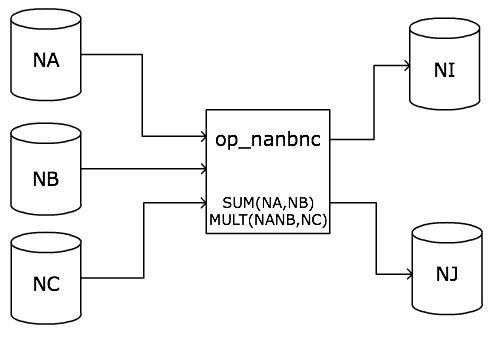
\includegraphics[width=7cm]{images/fig_ex3.jpg}
    \caption{Diagrama do experimento 3}
    \label{fig:ex3}
\end{figure}

Na figura \ref{fig:ex3} ilustra-se um fluxo de trabalho que utiliza como entrada de dados tr�s matrizes: $NA, NB$ e $NC$. O operador aplicado, $op_{\{na,nb,nc\}}$ soma as matrizes $NA$ e $NB$ e a matriz resultante � multiplicada com $NC$.

Apenas um n� ($h_1$) foi utilizado para a execu��o deste experimento. Os detalhes da execu��o est�o descritos na tabela \ref{tab:ex3}.

\begin{table}[ht]
	\centering
	\caption{Resultados do experimento com encadeamento de fluxos}
	\label{tab:ex3}
	\begin{tabular}{llll|l|}
	\hline
	\multicolumn{1}{|c|}{Ordem} & \multicolumn{1}{c|}{Host} & \multicolumn{1}{c|}{Operador} & \multicolumn{1}{c|}{Dados} & \multicolumn{1}{c|}{Tempo (ms)} \\ 
	\hline
	\multicolumn{1}{|c|}{1} & \multicolumn{1}{c|}{$h_1$} & \multicolumn{1}{c|}{SUM,MULT} & \multicolumn{1}{c|}{$NA,NB,NC$} & \multicolumn{1}{r|}{5809} \\ 
	\hline
	\multicolumn{1}{|c|}{2} & \multicolumn{1}{c|}{*} & \multicolumn{1}{c|}{DIFUNDIR} & \multicolumn{1}{c|}{$NI,NJ$} & \multicolumn{1}{r|}{7258} \\ 
	\hline
	\multicolumn{1}{|c|}{3} & \multicolumn{1}{c|}{*} & \multicolumn{1}{c|}{coletor de informa��o} & \multicolumn{1}{c|}{metadados} & \multicolumn{1}{r|}{91} \\ 
	\hline
	\multicolumn{4}{|c|}{tempo de planejamento} & \multicolumn{1}{r|}{1030} \\ 
	\hline
	\multicolumn{4}{|c|}{tempo de tradu��o} & \multicolumn{1}{r|}{580} \\ 
	\hline
	\multicolumn{4}{|c|}{tempo de difus�o} & \multicolumn{1}{r|}{7258} \\ 
	\hline
	\multicolumn{4}{|c|}{tempo processamento} & \multicolumn{1}{r|}{5809} \\ 
	\hline
	\multicolumn{4}{|c|}{tempo total} & \multicolumn{1}{r|}{14790} \\ 
	\hline
	\end{tabular}
\end{table}

\section{Considera��es}
\label{ex-consideracoes}

O principal experimento \ref{ex2} demonstra a capacidade do planejador adaptar o escalonamento de acordo com a situa��o dos recursos. Na primeira execu��o, quando os quatro n�s estavam dispon�veis, o melhor plano foi tra�ado, executando quatro operadores em paralelo $op_{\{h,i\}}$, $ op_{\{e,f\}}$, $op_{\{c,d\}}$ e $op_{\{a,b\}}$, gerando o plano de execu��o com dez passos. Ao trabalhar com um ambiente com um n� parcialmente ocupado, a primeira parte da execu��o foi escalonada com tr�s operadores. Entretanto, outras execu��es paralelas foram alocadas durante o plano deixando-o tamb�m com dez passos.

A utiliza��o da paraleliza��o direta mostra que o ambiente est� preparado para a adequa��o da paraleliza��o por plano, no qual o pr�prio planejador escolhe qual operador e quantos n�s ser�o utilizados para a execu��o de uma determinada tarefa.

No experimento que utiliza m�ltiplas entradas de dados, demonstra-se que sistema � capaz de agregar operadores mais elaborados, que utilizem v�rias opera��es e conjuntos de dados variados.

Os experimentos realizados neste trabalho foram direcionados para a valida��o do modelo (se��o \ref{modelo}). Para isto implementou-se e testou-se as principais funcionalidades para um ambiente de execu��o distribu�da com a gera��o de planos de execu��o por um planejador.

\section[Conclus�o]{Conclus�o}

\begin{frame}
    \frametitle{Conclus�o}
    \begin{itemize}
		\item proposta de um trabalho para execu��o de fluxos de trabalho cient�ficos;
		\item t�cnicas de planejamento:
		\begin{itemize}
			\item tempo de execu��o: estimado fornecido pelo usu�rio;
			\item coeficiente de tempo: execu��es anteriores;
			\item situa��o atual do ambiente distribu�do;
		\end{itemize}
		\item coeficiente de custos: utilizado pelo planejador para criar planos de execu��o;
		\item modulariza��o dos componentes do modelo;
		\item cen�rio flex�vel e expans�vel;
		\item modifica��o do \emph{PeerUnit}: gerenciador de execu��o;
		\item defini��o de um modelo de custos;
		\item uma limita��o do modelo: fluxos c�clicos;
		\begin{itemize}
			\item alternativa parcial: encapsular fluxo de trabalho (m�ltiplas entradas e sa�da de dados);
		\end{itemize}
	\end{itemize}
\end{frame}

\begin{frame}
    \frametitle{Trabalhos Futuros}
    \begin{itemize}
		\item refinamento do \emph{Or�culoDeMetaDados};
		\item utiliza��o de outras m�tricas:
		\begin{itemize}
			\item minimiza��o de gasto de energia;
			\item maximiza��o da utiliza��o de recursos;
		\end{itemize}
		\item m�todo de difus�o inteligente: capaz de analisar o plano e propagar os dados apenas para os n�s que utilizar�o tais dados;
		\item planejador capaz de escolher a melhor implementa��o de um operador para o plano a ser gerado:
		\item paraleliza��o por plano:
		\begin{itemize}
			\item n�o se fixa uma quantidade de n�s para cada fluxo de trabalho;
			\item de acordo com informa��es do \emph{Or�culoDeMetadados} planejador define o n�mero adequado para a paraleliza��o;
			\item necess�ria adapta��o do m�todo de tradu��o (considerar os n�s dispon�veis para cada tarefa);
		\end{itemize}
	\end{itemize}
\end{frame}

%%%%%%%%%%%%%%%%%%%%%%%%%%%%%%
% S L I D E S    F I N A I S %
%%%%%%%%%%%%%%%%%%%%%%%%%%%%%%

%\section[Refer�ncias]{Refer�ncias}
\begin{frame}[t,allowframebreaks]
    \frametitle{Refer�ncias}
    \nocite{*}
    \bibliographystyle{bst/sbc}
    \tiny \bibliography{bibliografia/bibliografia}
\end{frame}


\end{document}